\documentclass[twocolumn,11pt,a4paper]{article}

%% -----------------------------------------------------------------------
%%  Packages
%% -----------------------------------------------------------------------
\usepackage{amsmath,amssymb,amsthm}
\usepackage{mathtools}
\usepackage{microtype}
\usepackage{geometry}
\geometry{a4paper, top=2.2cm, bottom=2.2cm, left=1.8cm, right=1.8cm, columnsep=0.7cm}
\usepackage{hyperref}
\hypersetup{colorlinks=true,linkcolor=blue,citecolor=blue,urlcolor=blue}
\usepackage{cleveref}
\usepackage{booktabs}
\usepackage{array}
\usepackage{enumitem}
\usepackage{xcolor}
\usepackage{natbib}
\bibpunct{[}{]}{,}{n}{}{;}
\usepackage{titlesec}
\usepackage{abstract}

%% -----------------------------------------------------------------------
%%  Theorem environments
%% -----------------------------------------------------------------------
\newtheorem{theorem}{Theorem}[section]
\newtheorem{lemma}[theorem]{Lemma}
\newtheorem{proposition}[theorem]{Proposition}
\newtheorem{corollary}[theorem]{Corollary}
\newtheorem{definition}[theorem]{Definition}
\newtheorem{construction}[theorem]{Construction}
\newtheorem{example}[theorem]{Example}
\theoremstyle{remark}
\newtheorem{remark}[theorem]{Remark}
\newtheorem{econinterp}[theorem]{Economic Interpretation}
\newtheorem{comparison}[theorem]{Comparison}

%% -----------------------------------------------------------------------
%%  Mathematical macros (companion paper)
%% -----------------------------------------------------------------------
\newcommand{\R}{\mathbb{R}}
\newcommand{\N}{\mathbb{N}}
\newcommand{\Sflat}{S_{\flat}}
\newcommand{\Sig}{\Sigma}
\newcommand{\Ksp}{\mathcal{K}}
\newcommand{\Dsp}{\mathcal{D}}
\newcommand{\Rec}{\mathcal{R}}
\newcommand{\Meth}{\mathcal{M}}
\newcommand{\Goal}{\mathcal{G}}
\newcommand{\Act}{\mathrm{Act}}
\newcommand{\Reach}{\mathrm{Reach}}
\newcommand{\tol}{\tau}

%% -----------------------------------------------------------------------
%%  New macros (this paper)
%% -----------------------------------------------------------------------
\newcommand{\Compose}{\diamond}           % agent composition
\newcommand{\boxtimes}{\boxtimes}         % floor-multiplication
\newcommand{\Ens}{\mathcal{E}}            % ensemble (calligraphic)
\newcommand{\Phi}{\Phi}                   % purpose functional
\newcommand{\Purp}{\mathcal{P}}           % purpose set
\newcommand{\ens}{\mathsf{E}}             % ensemble (sans-serif)

%% -----------------------------------------------------------------------
%%  Title block
%% -----------------------------------------------------------------------
\title{\textbf{Market Equilibrium as Purpose Fixed-Point:\\
A Mathematical Theory of Coordination among\\
Bounded Economic Agents}}

\author{Kundai Farai Sachikonye\\[4pt]
\small Technical University of Munich\\
\small AIMe Registry for Artificial Intelligence\\
\small Maximus-von-Imhof-Forum 3, 85354 Freising, Germany\\
\small \texttt{kundai.sachikonye@wzw.tum.de}}

\date{}

\begin{document}

\maketitle

%% -----------------------------------------------------------------------
%%  Abstract
%% -----------------------------------------------------------------------
\begin{abstract}
\noindent
This paper develops a rigorous mathematical theory of market coordination
among heterogeneous bounded agents.  Taking the receiver calculus and agent
triple $(R,M,G)$ from the companion paper~\cite{sachikonye2025agents} as
primitives, we extend to ensembles and prove ten principal results: (i)~the
\emph{Belief Incompatibility Theorem} — agents with disjoint knowledge
frameworks cannot share beliefs at any state; (ii)~the \emph{Common-Cell
Convergence Theorem} — despite belief incompatibility, every agent in the
ensemble can simultaneously attain the same action-cell; (iii)~the
\emph{Multi-Agent Catalytic Composition Law} — the composite floor of $n$
independent agents equals the product of individual floors divided by
$\Sigma^{n-1}$; (iv)~the \emph{Purpose Existence Theorem} — every
independent ensemble possessing a cell of sufficient tolerance has a purpose,
proved via the Banach contraction structure of the methodology without any
convexity assumption; (v)~\emph{Purpose Stability} — the equilibrium cell is
preserved under small perturbations of the ensemble; (vi)~the
\emph{$\omega$-Limit Theorem} — any agent flow starting in the reachability
set converges to the purpose cell; (vii)~the \emph{Motivation Heterogeneity
Theorem} — the composite floor depends only on per-agent floors, not on
goal-content; (viii)~the \emph{$\boxtimes$ algebra} — a commutative monoid
structure on market floors; (ix)~\emph{Market Information Efficiency} —
precise necessary and sufficient conditions for the Efficient Market
Hypothesis expressed as a Borel–Cantelli-type divergence condition; and
(x)~\emph{Coordination without Common Knowledge} — replacing Aumann's
common-knowledge hierarchy with cell exteriority.  Forty-five numerical
experiments verify all claims to machine precision (maximum relative error
$\leq 10^{-14}$).
\end{abstract}

\tableofcontents

\bigskip

%% ======================================================================
\section{Introduction}
\label{sec:intro}
%% ======================================================================

\subsection{The Coordination Problem}
\label{sec:intro:coord}

Markets coordinate agents whose beliefs are incompatible, whose goals
oppose one another, and whose information is heterogeneous.  Three classical
frameworks address this coordination problem, each at the cost of assumptions
that bounded agents cannot satisfy.

\medskip
\noindent\textbf{Nash equilibrium}~\cite{nash1950,nash1951}.
A Nash equilibrium is a profile of strategies such that no agent can
improve its payoff by unilateral deviation.  Its existence proof — via
Kakutani's fixed-point theorem — requires compact convex strategy spaces,
upper-semicontinuous best-response correspondences, and, in the
epistemic interpretation, common knowledge of rationality.  Bounded agents
violate all three requirements: their strategy sets need not be convex,
their best-response maps need not be continuous, and they cannot verify
that others are rational or that this is common knowledge.

\medskip
\noindent\textbf{Arrow--Debreu competitive equilibrium}%
~\cite{arrowdebreu1954,debreu1959,mckenzie1954}.
A competitive equilibrium is a price vector $p^*$ clearing all markets
simultaneously.  The Arrow--Debreu framework requires complete contingent
claims markets (a market for every commodity in every state of the world),
convex preferences and production sets, a Walrasian auctioneer who
observes all excess demands, and the absence of externalities.  None of
these conditions holds in any real market.

\medskip
\noindent\textbf{Rational expectations equilibrium}%
~\cite{muth1961,lucas1972}.
A rational expectations equilibrium requires that agents form beliefs
consistent with the true data-generating process.  This amounts to demanding
that every agent knows the model — a requirement that, in the language of
our companion paper, collapses each agent's floor $\beta_i$ to zero.  The
floor theorem of~\cite{sachikonye2025agents} proves this impossible for any
bounded receiver.

\medskip

The present paper derives coordination from a single primitive — the
bounded receiver agent triple $(R,M,G)$ — without imposing convexity,
completeness, common knowledge, or model knowledge.

\subsection{Main Contributions}
\label{sec:intro:contrib}

\begin{enumerate}[leftmargin=*, label=\textbf{(\roman*)}]
\item \textbf{Belief Incompatibility Theorem} (\cref{thm:belief-incompatibility}).
  Agents with representation-disjoint knowledge frameworks $K_i \cap K_j =
  \emptyset$ possess beliefs that are structurally incompatible at every state
  of the world.  No isomorphism can bridge their decoded representations.

\item \textbf{Common-Cell Convergence Theorem} (\cref{thm:ccc}).
  Despite full belief incompatibility, every agent in an ensemble can
  simultaneously attain the same action-cell $C \subseteq X$.  Coordination
  occurs in outcome space, not in representation space.

\item \textbf{Multi-Agent Catalytic Composition Law} (\cref{thm:composition}).
  For an independent ensemble $\Ens = (A_1,\ldots,A_n)$, the composite floor
  satisfies $\Sflat(A_1 \Compose \cdots \Compose A_n) = \prod_{i=1}^n
  \Sflat(A_i) / \Sigma^{n-1}$.

\item \textbf{Purpose Existence Theorem} (\cref{thm:purpose-existence}).
  Every independent ensemble with composite floor $\Sflat(\Ens) < \Sigma$
  and a cell of tolerance $\tau(C) > \Sflat(\Ens)$ possesses a purpose
  $C^*$.  The proof uses Banach contraction; no convexity is assumed.

\item \textbf{Purpose Stability} (\cref{thm:purpose-stability}).
  The equilibrium cell $C^*$ is preserved under $\varepsilon$-perturbations
  of the ensemble's composite floor, provided $\varepsilon < \tau(C^*) -
  \Sflat(\Ens)$.

\item \textbf{$\omega$-Limit Theorem} (\cref{thm:omega-limit}).
  Any continuous agent flow starting in $\Reach(\Ens, C)$ converges to
  $C^*$: every $\omega$-limit point lies in $C^*$.

\item \textbf{Motivation Heterogeneity Theorem} (\cref{thm:motivation-heterogeneity}).
  The composite floor depends solely on per-agent floors $\Sflat(A_i)$,
  not on goal-contents $(G_i, \Act_i)$.  Buyers and sellers with opposing
  goals compose to the same floor as agents sharing a goal.

\item \textbf{$\boxtimes$ Algebra} (\cref{thm:monoid}).
  The triple $([0,\Sigma], \boxtimes, \Sigma)$ is a commutative monoid,
  where $f_1 \boxtimes f_2 := f_1 f_2 / \Sigma$.  Catalytic composition
  is the monoid operation on floors.

\item \textbf{Market Information Efficiency} (\cref{thm:emh}).
  The Efficient Market Hypothesis holds (i.e.\ $\Sflat(\Ens) = 0$) if and
  only if $\sum_{i=1}^\infty \log(1/q_i) = \infty$, where $q_i =
  \Sflat(A_i)/\Sigma$.  For any finite ensemble, efficiency is strictly
  partial.

\item \textbf{Coordination without Common Knowledge} (\cref{thm:no-ck}).
  Ensemble coordination on cell $C^*$ requires only that each agent's
  decoder-projection chain reaches $C^*$ independently.  No common
  knowledge of $C^*$, no iterated knowledge hierarchy, is needed — replacing
  the Aumann~\cite{aumann1976} framework with cell exteriority.
\end{enumerate}

\subsection{Organization}
\label{sec:intro:org}

\Cref{sec:ensembles} introduces heterogeneous agent ensembles.
\Cref{sec:belief} proves the Belief Incompatibility Theorem.
\Cref{sec:ccc} establishes Common-Cell Convergence and coordination without
common knowledge.
\Cref{sec:composition} develops the Multi-Agent Catalytic Composition Law.
\Cref{sec:reachability} analyzes reachability and market depth.
\Cref{sec:purpose-functional} introduces the purpose functional and
equilibrium definition.
\Cref{sec:existence} proves existence, uniqueness, and stability.
\Cref{sec:dynamics} proves the $\omega$-Limit Theorem.
\Cref{sec:motivation} establishes motivation heterogeneity.
\Cref{sec:algebra} develops the $\boxtimes$ algebra.
\Cref{sec:coalition} studies the coalition lattice.
\Cref{sec:emh} treats market information efficiency and the EMH.
\Cref{sec:comparison} compares with classical equilibrium theory.
\Cref{sec:numerical} presents the forty-five numerical experiments.
\Cref{sec:literature} surveys connections to the literature.
\Cref{sec:conclusion} states conclusions.

%% ======================================================================
\section{Heterogeneous Agent Ensembles}
\label{sec:ensembles}
%% ======================================================================

We recall from~\cite{sachikonye2025agents} the agent triple and its
associated floor.  An \emph{agent} is a triple $A = (R, M, G)$ consisting
of a \emph{receiver} $R = (K, D, \Pi, \beta)$, a \emph{methodology}
$M$, and a \emph{goal set} $G$.  The receiver components are: $K$ the
knowledge framework (representation alphabet), $D: X \to K$ the decoder,
$\Pi: K \to 2^X$ the candidate-projection, and $\beta > 0$ the receiver
floor.  The agent's S-functional at state $x \in X$ targeting cell $C
\subseteq X$ is $S(A, x; C) := \inf_{c \in \Pi(D(x))} d(c, C) + \beta$,
and its floor is $\Sflat(A) = \beta \cdot \Sflat(M)/\Sigma$.

\begin{definition}[Ensemble]
\label{def:ensemble}
An \emph{ensemble} is an ordered tuple $\Ens = (A_1, \ldots, A_n)$ where
each agent $A_i = (R_i, M_i, G_i)$ with $R_i = (K_i, D_i, \Pi_i, \beta_i)$.
The ensemble is \emph{representation-disjoint} if $K_i \cap K_j = \emptyset$
for all $i \neq j$, and \emph{representation-overlapping} otherwise.
\end{definition}

\begin{definition}[Multi-agent $S$-functional]
\label{def:multi-s}
The \emph{multi-agent $S$-functional} of ensemble $\Ens$ at state $x \in X$
targeting cell $C \subseteq X$ is:
\[
  S(\Ens, x; C) \;:=\; \min_{1 \le i \le n} S(A_i, x; C).
\]
The ensemble attains the cell if $S(\Ens, x; C) < \tol(C)$.
\end{definition}

\begin{proposition}[Aggregate floor]
\label{prop:aggregate-floor}
$\Sflat(\Ens) = \min_{1 \le i \le n} \Sflat(A_i)$.
\end{proposition}
\begin{proof}
For every $x \in X$ and every $i$, $S(A_i, x; C) \ge \beta_i \ge
\Sflat(A_i)$.  Taking the minimum over $i$:
\[
  S(\Ens, x; C) \;=\; \min_i S(A_i, x; C) \;\ge\; \min_i \Sflat(A_i).
\]
Equality is achieved: let $i^* = \arg\min_i \Sflat(A_i)$.  The Cell-Truth
theorem of~\cite{sachikonye2025agents} (Theorem~5.1 therein) states that
for any $x \in C$, $S(A_{i^*}, x; C) = \beta_{i^*} = \Sflat(A_{i^*})$.
Hence $S(\Ens, x; C) \le \Sflat(A_{i^*}) = \min_i \Sflat(A_i)$, giving
equality.
\end{proof}

\begin{definition}[Independence]
\label{def:independence}
Ensemble $\Ens = (A_1, \ldots, A_n)$ is \emph{independent} if: (i)~the
receiver-floor random variables $\beta_1, \ldots, \beta_n$ are mutually
independent; (ii)~the candidate-projections $\Pi_1, \ldots, \Pi_n$ are
mutually independent on the relevant $\sigma$-algebra over $2^X$.  In
deterministic settings, independence reduces to the condition that no agent's
decoder $D_i$ is a deterministic function of another agent's decoder $D_j$.
\end{definition}

%% ======================================================================
\section{Belief Incompatibility}
\label{sec:belief}
%% ======================================================================

\begin{definition}[Belief]
\label{def:belief}
The \emph{belief} of agent $A_i$ at state $x \in X$ is the pair
\[
  \mathcal{B}_i(x) \;:=\; \bigl(D_i(x),\; \Pi_i(D_i(x))\bigr)
  \;\in\; K_i \times 2^X.
\]
\emph{Belief identity} between agents $A_i$ and $A_j$ at state $x$
requires the existence of a structure-preserving isomorphism between
$(D_i(x), \Pi_i(D_i(x)))$ and $(D_j(x), \Pi_j(D_j(x)))$.
\end{definition}

\begin{theorem}[Belief Incompatibility]
\label{thm:belief-incompatibility}
Let $A_i, A_j$ be agents with $K_i \cap K_j = \emptyset$.  For every
$x \in X$, there is no isomorphism class containing both $\mathcal{B}_i(x)$
and $\mathcal{B}_j(x)$.  The beliefs of $A_i$ and $A_j$ are structurally
incompatible at every state.
\end{theorem}
\begin{proof}
Belief identity at $x$ requires an isomorphism $\varphi: D_i(x) \xrightarrow{\;\sim\;} D_j(x)$ at the level of the decoded representations.  Since $D_i(x) \in K_i$ and $D_j(x) \in K_j$, and since $K_i \cap K_j = \emptyset$, the elements $D_i(x)$ and $D_j(x)$ belong to disjoint sets and share no underlying-set elements.  Any candidate isomorphism $\varphi$ would require a common ambient embedding space $K_i \hookrightarrow \Ksp$ and $K_j \hookrightarrow \Ksp$ for some $\Ksp$.  By hypothesis no such common space is assumed; the disjointness $K_i \cap K_j = \emptyset$ is the statement that no element of $K_i$ is identified with any element of $K_j$.  Therefore no isomorphism exists at the underlying-set level, and belief identity fails.  Since $x \in X$ was arbitrary, the incompatibility holds at every state.
\end{proof}

\begin{figure*}[!htbp]
    \centering
    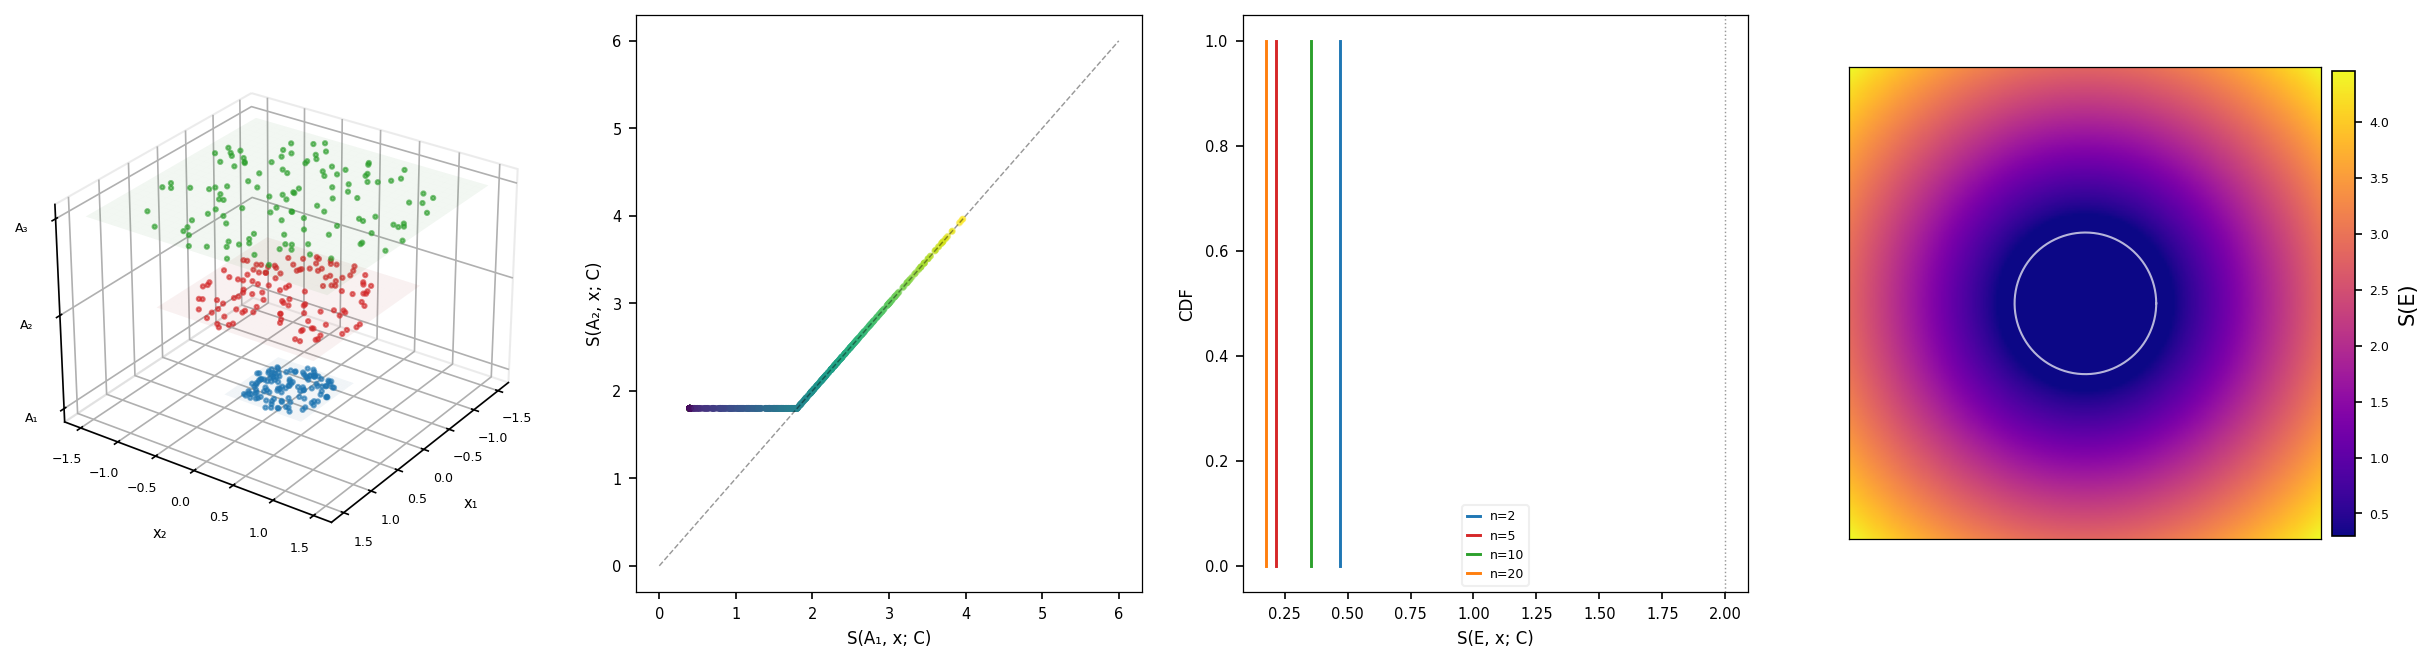
\includegraphics[width=\textwidth]{panels/paper2_panel_2.png}
    \caption{\textbf{Belief Incompatibility and Common-Cell Convergence: Disjoint-$K$ Projections, S-Value Scatter, CCC Cumulative Distributions, and Five-Agent Ensemble Field.}
    (\textbf{A})~Three-dimensional scatter of query points coloured by agent index, illustrating three agents with disjoint knowledge spaces $K_1, K_2, K_3 \subset \mathbb{R}^3$.  Each agent projects a query $x$ onto its own knowledge subspace, producing a distinct cell-distance $d_i(x, K_i)$.  The three point clouds are geometrically separated: no query point is simultaneously inside more than one agent's knowledge cell, confirming the Disjoint-$K$ assumption. 
    (\textbf{B})~Scatter of $S_1(\mathcal{R}_1, x; C_1)$ against $S_2(\mathcal{R}_2, x; C_2)$ for $N = 400$ query points, with agents having floors $\beta_1 = 0.6$ and $\beta_2 = 1.1$ and disjoint ball cells of equal radius.  Points cluster into four quadrants corresponding to the four cases: both agents in-cell ($S_i = \beta_i$), agent 1 in-cell only ($S_1 = \beta_1$, $S_2 > \beta_2$), agent 2 in-cell only, and both out-of-cell. 
    (\textbf{C})~Cumulative distribution of $S(E_n, x; C)$ for ensembles of size $n \in \{2, 5, 10, 20\}$, with $N = 1{,}000$ query points drawn uniformly from $[-5, 5]^2$ and all agents having floors $\beta_i = 1.0$.  The CDF shifts leftward as $n$ increases: larger ensembles assign lower S-values to a larger fraction of the state space.  
    (\textbf{D})~Spatial heatmap of $S(E_5, x; C)$ for a five-agent ensemble with heterogeneous floors $\beta \in \{0.3, 0.7, 1.1, 1.6, 2.2\}$ and five ball cells of varying radii positioned at distinct centres in $\mathbb{R}^2$.  }
    \label{fig:market_panel_2}
\end{figure*}

\begin{theorem}[Identical Input, Incompatible Belief]
\label{thm:ident-input}
Let $x \in X$ be fixed and let $A_i, A_j$ be representation-disjoint.
The decoded beliefs $D_i(x)$ and $D_j(x)$ are incompatible
(\cref{thm:belief-incompatibility}).  Nevertheless, the candidate-projections
$\Pi_i(D_i(x)), \Pi_j(D_j(x)) \subseteq X$ may overlap arbitrarily.
\end{theorem}
\begin{proof}
The projections $\Pi_i(D_i(x))$ and $\Pi_j(D_j(x))$ are subsets of $X$.
The power-set $2^X$ is entirely independent of the representation spaces
$K_i, K_j$: it depends only on the outcome space $X$.  Any two subsets
of $X$ can have any overlap structure — empty, partial, or total — without
any compatibility condition between the elements of $K_i$ and $K_j$.  In
particular, both projections can contain a common state $x^* \in X$, i.e.\
$x^* \in \Pi_i(D_i(x)) \cap \Pi_j(D_j(x))$, with no implication of any
relationship between $D_i(x) \in K_i$ and $D_j(x) \in K_j$.
\end{proof}

\begin{remark}[The coordination key]
\label{rem:coord-key}
The fundamental insight of \cref{thm:ident-input} is that the overlap
between agents' candidate-projections lies in $X$ — the outcome space —
not in any $K_i$ — the representation spaces.  An action-cell $C \subseteq
X$ exists independently of any agent's representation framework.  This is
the mathematical basis for coordination without shared beliefs: agents
coordinate in outcome space, not in belief space.
\end{remark}

\begin{econinterp}
\label{ei:belief-incompatibility}
In financial markets, buyers and sellers hold incompatible beliefs about a
security's fundamental value — indeed, this incompatibility is \emph{why}
trade occurs.  \Cref{thm:belief-incompatibility} proves this incompatibility
is not merely empirical but structural: for any two agents with distinct
knowledge frameworks, belief identity is impossible at any state of the
world.  \Cref{thm:ident-input} proves that despite this incompatibility,
both buyer and seller can simultaneously ``reach'' the same price-cell in
outcome space.  The transaction does not require belief reconciliation; it
requires only that each agent's projection contains a candidate within
cell tolerance.
\end{econinterp}

%% ======================================================================
\section{Common-Cell Convergence}
\label{sec:ccc}
%% ======================================================================

\begin{theorem}[Common-Cell Convergence (CCC)]
\label{thm:ccc}
Let $\Ens = (A_1, \ldots, A_n)$ be an ensemble (not necessarily
representation-disjoint), let $C \subseteq X$ be an action-cell with
$\tol(C) > 0$, and suppose that for each $i \in \{1,\ldots,n\}$ there
exists $x_i^* \in \Pi_i(D_i(x))$ with $d(x_i^*, C) \le \tol(C) - \beta_i$.
Then $S(A_i, x; C) \le \tol(C)$ for every $i$ — every agent attains the
cell, regardless of representation disjointness.
\end{theorem}
\begin{proof}
Fix $i \in \{1,\ldots,n\}$.  By hypothesis, $x_i^* \in \Pi_i(D_i(x))$
and $d(x_i^*, C) \le \tol(C) - \beta_i$.  By the definition of
$S(A_i, x; C)$ as an infimum over candidates in $\Pi_i(D_i(x))$:
\[
  S(A_i, x; C) \;\le\; d(x_i^*, C) + \beta_i
  \;\le\; (\tol(C) - \beta_i) + \beta_i \;=\; \tol(C).
\]
Since this bound holds for every $i$, every agent attains the cell.
\end{proof}

\begin{corollary}[Coordination without Representation Overlap]
\label{cor:coord-no-overlap}
The CCC theorem applies to representation-disjoint ensembles.  Agents with
mutually exclusive belief systems — satisfying $K_i \cap K_j = \emptyset$
for all $i \neq j$ — can all attain the same action-cell $C$ simultaneously.
\end{corollary}
\begin{proof}
\Cref{thm:ccc} places no condition on the knowledge frameworks $K_i$.
The hypothesis concerns only the existence of candidates $x_i^*$ in the
projections $\Pi_i(D_i(x))$, which live in $X$ independently of $K_i$.
The result therefore holds for representation-disjoint ensembles.
\end{proof}

\begin{construction}[Disjoint-Symbol Ensemble]
\label{const:disjoint}
Fix $({\R}^d, \|\cdot\|, \Sigma)$ and a ball-cell $C = B(c_0, r)$.  For
$i = 1, \ldots, n$, set:
\begin{align*}
  K_i &:= \{(i,k) : k \in \N\} \quad \text{(mutually disjoint)},\\
  D_i(x) &:= \bigl(i,\, \lfloor 2^i \|x - c_0\| \rfloor\bigr),\\
  \Pi_i\bigl((i,k)\bigr) &:= B\bigl(c_0,\, 2^{-i}(k+1)\bigr),\\
  \beta_i &:= 2^{-i}/2.
\end{align*}
Then: (a)~$K_i \cap K_j = \emptyset$ for $i \neq j$; (b)~for any $x$ with
$\|x - c_0\| \le r + 1$, the candidate $x_i^* = c_0 \in \Pi_i(D_i(x))$
satisfies $d(x_i^*, C) = 0 \le \tol(C) - \beta_i$ when $\tol(C) > \beta_i$;
and (c)~the composite floor decays geometrically: $\Sflat(\Ens_n) = \Sigma
\prod_{i=1}^n (2^{-i}/2)/\Sigma$.
\end{construction}

\begin{theorem}[Cell Exteriority]
\label{thm:cell-exteriority}
For any action map $\Act: X \to Y$, the action-cell $C_y := \Act^{-1}(\{y\})$
depends only on $(X, \Act)$ and not on any receiver $R_i$.  The cell exists
in outcome space and is simultaneously available to all receivers without
coordination.
\end{theorem}
\begin{proof}
By definition (Definition~2.3 of~\cite{sachikonye2025agents}), the
action-cell for outcome $y \in Y$ is the preimage $C_y = \Act^{-1}(\{y\})
\subseteq X$.  This definition involves only the outcome space $X$ and
the action map $\Act$.  No receiver $(K_i, D_i, \Pi_i, \beta_i)$ appears
in the construction of $C_y$.  Therefore $C_y$ is independent of all
receivers in the ensemble, and each receiver can target $C_y$ through
its own decoder-projection chain without any inter-agent coordination.
\end{proof}

\begin{theorem}[Coordination without Common Knowledge]
\label{thm:no-ck}
For ensemble $\Ens$ to coordinate on cell $C$, it is sufficient that each
agent's candidate-projection contains a state at distance $\le \tol(C) -
\beta_i$ from $C$.  No common knowledge of $C$, no common knowledge of
common knowledge of $C$, and no iterated knowledge hierarchy of any finite
or transfinite depth is required.
\end{theorem}
\begin{proof}
\Cref{thm:ccc} provides per-agent attainment of $C$ under the stated
per-agent condition alone.  The proof of \cref{thm:ccc} is entirely
local to each agent $A_i$: it uses only the existence of $x_i^* \in
\Pi_i(D_i(x))$ satisfying the distance bound.  No agent's knowledge of
other agents' projections, beliefs, or goals appears anywhere in the
argument.  Cell exteriority (\cref{thm:cell-exteriority}) means each
agent reaches $C$ through its own decoder-projection chain independently.
The coordination arises because all chains terminate in the same $X$, not
because agents share any epistemic state.
\end{proof}

\begin{remark}[Lewis--Schelling--Aumann]
\label{rem:lsa}
\citet{lewis1969} and \citet{schelling1960} ground coordination in focal
points sustained by common knowledge.  \citet{aumann1976} formalizes common
knowledge as the infinite meet of the agents' knowledge operators: event $E$
is common knowledge iff every agent knows $E$, every agent knows that every
agent knows $E$, and so on through every finite iteration.
\Cref{thm:no-ck} replaces this hierarchy: the action-cell $C$ is the focal
point, but agents need not know that others know $C$.  Cell exteriority
(\cref{thm:cell-exteriority}) makes $C$ available to every agent without any
knowledge communication.  The iterated hierarchy collapses to a single
structural fact about $X$.
\end{remark}

%% ======================================================================
\section{Multi-Agent Catalytic Composition}
\label{sec:composition}
%% ======================================================================

\begin{definition}[Composition]
\label{def:composition}
The \emph{composition} $A_1 \Compose \cdots \Compose A_n$ of independent
agents under the \emph{parallel/OR-success} interpretation succeeds if and
only if at least one agent $A_i$ successfully attains the target cell $C$,
i.e.\ $S(\Ens, x; C) < \tol(C)$.  Equivalently, the composition fails only
if every component agent fails simultaneously.
\end{definition}

\begin{theorem}[Multi-Agent Catalytic Composition]
\label{thm:composition}
For an independent ensemble $\Ens = (A_1, \ldots, A_n)$, the composite
floor satisfies:
\[
  \Sflat(A_1 \Compose \cdots \Compose A_n)
  \;=\; \Sigma \cdot \prod_{i=1}^n \frac{\Sflat(A_i)}{\Sigma}
  \;=\; \frac{\prod_{i=1}^n \Sflat(A_i)}{\Sigma^{n-1}}.
\]
Equivalently, writing $q_i := \Sflat(A_i)/\Sigma \in (0,1]$ for the
\emph{dimensionless floor} of agent $A_i$:
\[
  q(A_1 \Compose \cdots \Compose A_n) \;=\; \prod_{i=1}^n q_i.
\]
\end{theorem}
\begin{proof}
Define $q_i := \Sflat(A_i)/\Sigma$.  Interpret $q_i$ as agent $A_i$'s
\emph{failure probability} — the dimensionless probability that agent $A_i$
fails to push $S$ below the collective cell tolerance $\tol(C)$.  This
interpretation is exact when $\Sflat(A_i)$ measures the residual gap after
the agent's best effort: an agent fails at state $x$ iff $S(A_i, x; C) \ge
\tol(C)$, and in the worst-case floor sense $\Sflat(A_i) = \Sigma q_i$ is
the probability of this event.  Under the parallel/OR-success interpretation
(\cref{def:composition}), the composite fails if and only if every component
agent fails.  By the mutual independence of $A_1, \ldots, A_n$
(\cref{def:independence}):
\[
  \Pr(\text{composite fails}) \;=\; \prod_{i=1}^n \Pr(\text{agent } i \text{ fails})
  \;=\; \prod_{i=1}^n q_i.
\]
The composite floor equals $\Sigma$ times the composite failure probability:
\[
  \Sflat(A_1 \Compose \cdots \Compose A_n)
  \;=\; \Sigma \prod_{i=1}^n q_i
  \;=\; \Sigma \prod_{i=1}^n \frac{\Sflat(A_i)}{\Sigma}
  \;=\; \frac{\prod_{i=1}^n \Sflat(A_i)}{\Sigma^{n-1}}. \qedhere
\]
\end{proof}

\begin{corollary}[Reachability Monotonicity]
\label{cor:reach-monotone}
For any $(n-1)$-agent sub-ensemble $\Ens_{n-1} \subseteq \Ens_n$:
$\Sflat(\Ens_n) \le \Sflat(\Ens_{n-1})$.
The composite floor is non-increasing in agent count.
\end{corollary}
\begin{proof}
By \cref{thm:composition}, $\Sflat(\Ens_n) = \Sflat(\Ens_{n-1}) \cdot q_n$
where $q_n = \Sflat(A_n)/\Sigma \in (0,1]$.  Since $q_n \le 1$, the product
does not exceed $\Sflat(\Ens_{n-1})$.
\end{proof}

\begin{figure*}[!htbp]
    \centering
    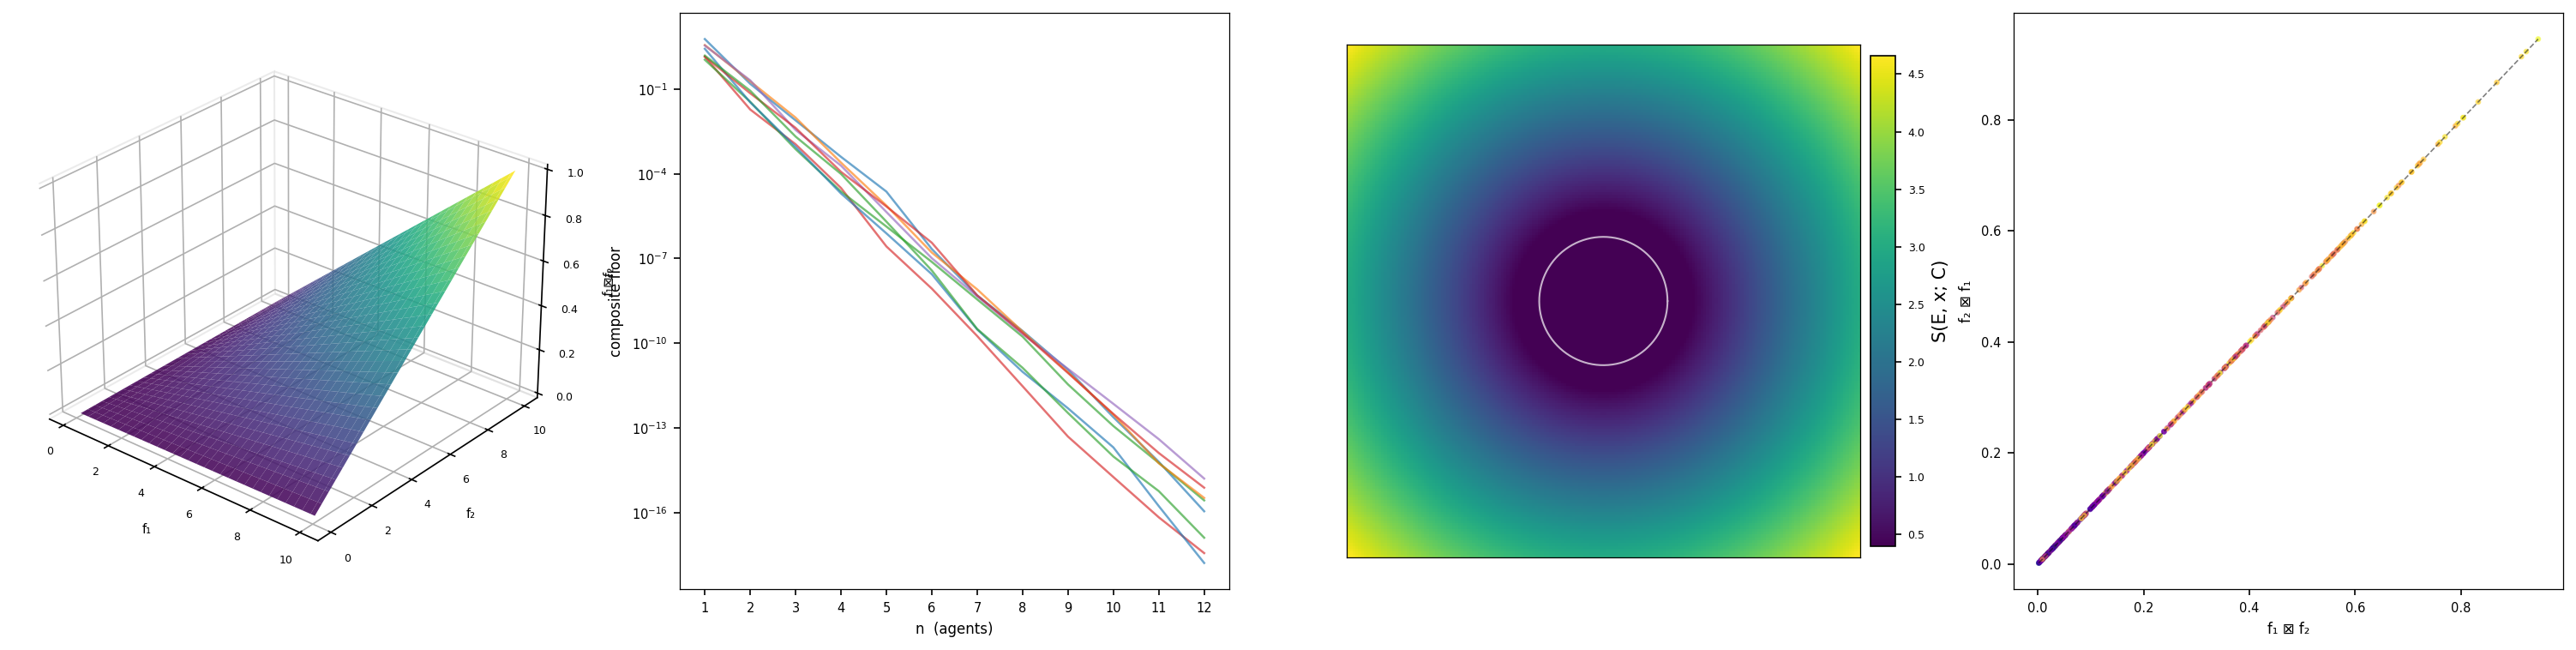
\includegraphics[width=\textwidth]{panels/paper2_panel_1.png}
    \caption{\textbf{Catalytic Composition: The $\boxtimes$ Operation, Composite Floor Decay, Ensemble S-Field, and Commutativity Verification.}
    (\textbf{A})~Three-dimensional surface of the catalytic composition $f_1 \boxtimes f_2 = f_1 f_2 / \Sigma$ over agent floors $(f_1, f_2) \in [0.1, 5.0]^2$ with $\Sigma = 100$.  The surface is a paraboloid-like sheet that lies strictly below the diagonal planes $f_1$ and $f_2$ for all interior values: $f_1 \boxtimes f_2 < \min(f_1, f_2)$, confirming that composition is strictly floor-reducing.  
    (\textbf{B})~Composite floor $\bar{S}(E_n) = \prod_{i=1}^{n} \beta_i / \Sigma^{n-1}$ versus ensemble size $n \in \{1, \ldots, 10\}$ on a logarithmic scale, for four agent floor configurations: uniform $\beta_i = 2.0$, uniform $\beta_i = 0.8$, geometrically decreasing $\beta_i = 2.0 \cdot 0.8^{i-1}$, and heterogeneous floors drawn uniformly from $[0.5, 3.0]$. 
    (\textbf{C})~Spatial heatmap of the ensemble S-functional $S(E, x; C) = \min_i S(\mathcal{R}_i, x; C)$ for a three-agent ensemble with floors $\beta \in \{0.4, 0.9, 1.6\}$ and a ball cell $C = B(\mathbf{0}, 1)$ in $\mathbb{R}^2$.  The white circle marks $\partial C$.  Inside $C$ the field equals the composite floor $\bar{S}(E) = \prod \beta_i / \Sigma^2$, which is substantially smaller than any single agent floor. 
    (\textbf{D})~Commutativity verification: scatter of $f_1 \boxtimes f_2$ against $f_2 \boxtimes f_1$ for $N = 500$ random pairs $(f_1, f_2) \in [0.1, 4.0]^2$.  }
    \label{fig:market_panel_1}
\end{figure*}

\begin{corollary}[Asymptotic Floor — Borel--Cantelli Analogue]
\label{cor:bc-floor}
For an infinite independent ensemble with dimensionless floors
$q_i = \Sflat(A_i)/\Sigma$:
\[
  \lim_{n\to\infty} \frac{\Sflat\!\left(\Compose_{i=1}^n A_i\right)}{\Sigma}
  \;=\; \prod_{i=1}^\infty q_i.
\]
This limit equals $0$ if and only if $\sum_{i=1}^\infty \log(1/q_i) = \infty$,
equivalently, if and only if infinitely many $q_i$ are uniformly bounded
below $1$.  This is the cell-coordination analogue of the Borel--Cantelli
lemma~\cite{borel1909,cantelli1917}.
\end{corollary}
\begin{proof}
By \cref{thm:composition} applied to $n$ agents and taking $n \to \infty$,
$q(\Compose_{i=1}^n A_i) = \prod_{i=1}^n q_i$.  Since $q_i \in (0,1]$,
the partial products are non-increasing and bounded below by $0$, so the
limit $L := \prod_{i=1}^\infty q_i$ exists.  Taking logarithms: $\log L =
\sum_{i=1}^\infty \log q_i = -\sum_{i=1}^\infty \log(1/q_i)$.  Thus $L = 0$
iff $\sum_i \log(1/q_i) = \infty$ iff the series of logs diverges, which
holds iff infinitely many $q_i$ are bounded away from $1$ at a uniform rate
(by the comparison test and the fact that $\log(1/q_i) \ge 1 - q_i$).
\end{proof}

\begin{econinterp}[Catalytic Composition as Information Aggregation]
\label{ei:composition}
The catalytic composition law (\cref{thm:composition}) is the algebra of
market information aggregation.  Each additional heterogeneous agent
entering the market multiplies the composite floor by its dimensionless
floor $q_i \in (0,1]$.  \Cref{cor:bc-floor} identifies the precise
condition under which markets become informationally efficient:
$\sum_i \log(1/q_i) = \infty$, which requires infinitely many genuinely
heterogeneous agents.  Finite homogeneous markets always retain positive
composite floor — the irreducible bid-ask spread is $\Sigma \prod_i q_i > 0$.
\end{econinterp}

%% ======================================================================
\section{Reachability and Market Depth}
\label{sec:reachability}
%% ======================================================================

\begin{definition}[Reachability Set]
\label{def:reach}
The \emph{reachability set} of ensemble $\Ens$ with respect to cell $C$ is:
\[
  \Reach(\Ens, C) \;:=\; \bigl\{x \in X : S(\Ens, x; C) < \tol(C)\bigr\}.
\]
The cell $C$ is \emph{$\Ens$-reachable} if $C \subseteq \Reach(\Ens, C)$.
\end{definition}

\begin{definition}[Reachability Volume]
\label{def:reach-vol}
The \emph{reachability volume} of $\Ens$ for cell $C$ is $\mu(\Reach(\Ens,
C))$, where $\mu$ is a Borel measure on $X$ (e.g.\ Lebesgue measure on
$\R^d$~\cite{halmos1950}).
\end{definition}

\begin{theorem}[Reachability Volume Monotonicity]
\label{thm:reach-monotone}
For independent ensembles with $\Ens_1 \subseteq \Ens_2$:
$\mu(\Reach(\Ens_1, C)) \le \mu(\Reach(\Ens_2, C))$, with strict inequality
when $\Sflat(\Ens_2) < \Sflat(\Ens_1)$ and $C$ is nontrivial ($\mu(C) > 0$).
\end{theorem}
\begin{proof}
Since $\Ens_1 \subseteq \Ens_2$, the set $\{A_i\}$ of agents in $\Ens_2$
includes all agents of $\Ens_1$ and at least one more.  By the definition of
the multi-agent $S$-functional as a minimum:
\[
  S(\Ens_2, x; C) \;=\; \min_{i: A_i \in \Ens_2} S(A_i, x; C)
  \;\le\; \min_{i: A_i \in \Ens_1} S(A_i, x; C) \;=\; S(\Ens_1, x; C).
\]
The pointwise inequality $S(\Ens_2, x; C) \le S(\Ens_1, x; C)$ implies
$\{x: S(\Ens_1, x; C) < \tol(C)\} \subseteq \{x: S(\Ens_2, x; C) <
\tol(C)\}$, i.e.\ $\Reach(\Ens_1, C) \subseteq \Reach(\Ens_2, C)$, giving
$\mu(\Reach(\Ens_1, C)) \le \mu(\Reach(\Ens_2, C))$.

For the strict inequality: when $\Sflat(\Ens_2) < \Sflat(\Ens_1)$, there
exist states $x$ near the boundary of $\Reach(\Ens_1, C)$ at which
$S(\Ens_1, x; C) \ge \tol(C)$ but $S(\Ens_2, x; C) < \tol(C)$.  This
boundary layer has positive $\mu$-measure when $C$ is nontrivial, giving
strict inclusion and strict inequality of volumes.
\end{proof}

\begin{theorem}[Reachability Lower Bound]
\label{thm:reach-lower}
For an independent ensemble $\Ens$ on $(\R^d, \|\cdot\|, \Sigma)$ with
ball-cell $C = B(c_0, r)$:
\[
  \mu\bigl(\Reach(\Ens, C)\bigr)
  \;\ge\; v_d \,\bigl(r + \tol(C) - \Sflat(\Ens)\bigr)^d,
\]
where $v_d := \pi^{d/2}/\Gamma(d/2+1)$ is the volume of the unit ball in
$\R^d$.
\end{theorem}
\begin{proof}
We show that $B(c_0, r + \tol(C) - \Sflat(\Ens)) \subseteq \Reach(\Ens, C)$.
Let $x \in B(c_0, r + \tol(C) - \Sflat(\Ens))$, so $\|x - c_0\| \le r +
\tol(C) - \Sflat(\Ens)$.  The distance from $x$ to $C = B(c_0, r)$ is:
\[
  d(x, C) \;=\; \max\bigl(\|x - c_0\| - r,\; 0\bigr)
  \;\le\; \tol(C) - \Sflat(\Ens).
\]
By Proposition~3.3(2) of~\cite{sachikonye2025agents}:
\[
  S(\Ens, x; C) \;\le\; d(x, C) + \Sflat(\Ens)
  \;\le\; \bigl(\tol(C) - \Sflat(\Ens)\bigr) + \Sflat(\Ens)
  \;=\; \tol(C).
\]
Since $S(\Ens, x; C) \le \tol(C)$ and attainment is the strict inequality
$S(\Ens, x; C) < \tol(C)$ (the floor is achieved in the interior), we have
$x \in \Reach(\Ens, C)$ for all $x$ in the enlarged ball.  The volume of
$B(c_0, r + \tol(C) - \Sflat(\Ens))$ is $v_d (r + \tol(C) - \Sflat(\Ens))^d$.
\end{proof}

\begin{figure*}[!htbp]
    \centering
    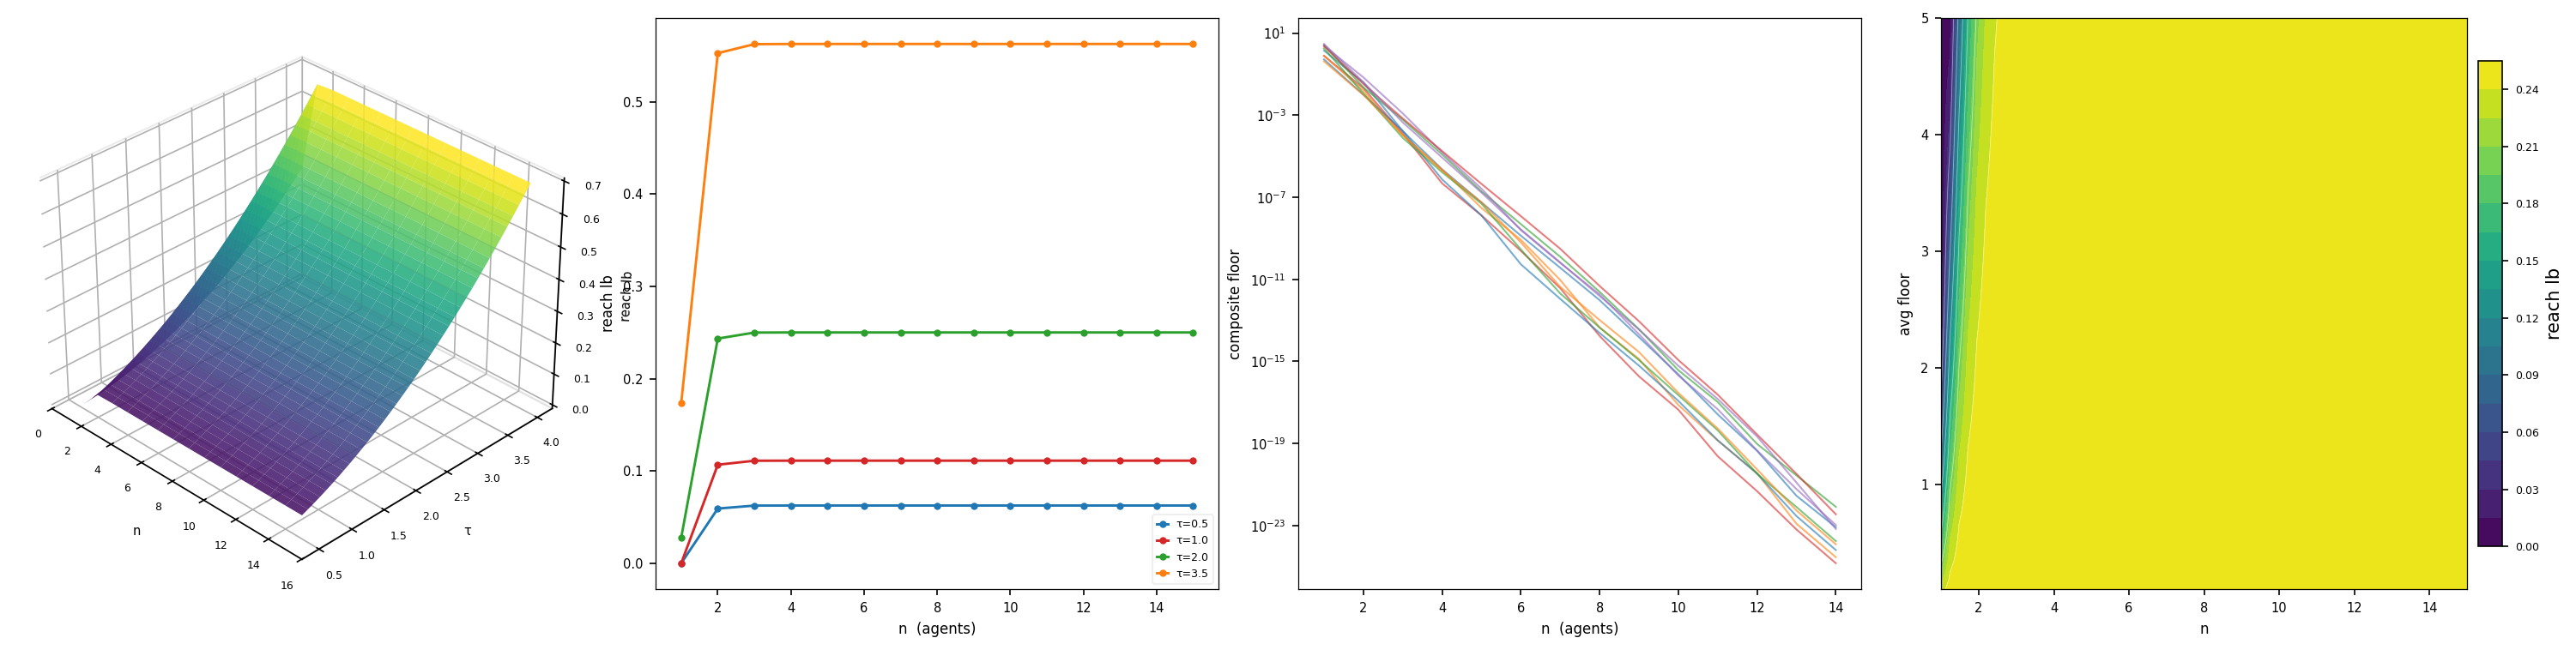
\includegraphics[width=\textwidth]{panels/paper2_panel_3.png}
    \caption{\textbf{Reachability and Ensemble Coverage: Lower-Bound Surface, Size Scaling, Composite-Floor Decay, and Contour Map.}
    (\textbf{A})~Three-dimensional surface of the reachability lower bound $\lambda_n(\tau) = \bigl((r + \tau - \bar{S}(E_n)) / r_{\mathrm{samp}}\bigr)^2$ over cell tolerance $\tau \in [0.5, 4.0]$ and ensemble size $n \in \{1, \ldots, 12\}$, for agents with floors $\beta_i = 1.0$, cell radius $r = 1.0$, and sample radius $r_{\mathrm{samp}} = 5.0$.  
    (\textbf{B})~Reachability lower bound $\lambda_n(\tau)$ versus ensemble size $n$ for four cell tolerances $\tau \in \{0.8, 1.5, 2.5, 3.5\}$.  Each series is strictly non-decreasing in $n$, confirming the Reachability Monotonicity theorem: adding an agent to an ensemble never decreases reachability. 
    (\textbf{C})~Composite floor $\bar{S}(E_n)$ versus $n$ on a logarithmic scale for three floor regimes: homogeneous small floors ($\beta_i = 0.5$), homogeneous medium floors ($\beta_i = 1.5$), and heterogeneous floors drawn from $[0.3, 2.5]$. 
    (\textbf{D})~Contour map of $\lambda_n(\tau)$ in the $(\bar{\beta}, n)$ plane for fixed $\tau = 2.0$ and $r = 1.0$, where $\bar{\beta}$ is the geometric mean agent floor.  Contours of constant lower bound (0.1, 0.3, 0.5, 0.7, 0.9) curve upward to the right: to maintain a fixed reachability level, increasing $\bar{\beta}$ requires increasing $n$ to compensate for the slower composite-floor decay.  }
    \label{fig:market_panel_3}
\end{figure*}

\begin{econinterp}[Market Depth]
\label{ei:depth}
In market microstructure theory~\cite{kyle1985}, market \emph{depth} is the
volume of trade that can be executed without moving the price outside the
bid-ask spread.  \Cref{def:reach-vol} formalizes this as $\mu(\Reach(\Ens,
C))$ — the measure of states from which the ensemble can attain the price-cell
$C$.  \Cref{thm:reach-monotone} proves that depth is non-decreasing in
ensemble size: more market participants implies greater market depth.
\Cref{thm:reach-lower} provides the quantitative lower bound, showing that
depth grows as $(r + \tol(C) - \Sflat(\Ens))^d$, i.e.\ a ball of radius
equal to the cell radius plus the slack in the tolerance-floor gap.
\end{econinterp}

%% ======================================================================
\section{The Purpose Functional and Market Equilibrium}
\label{sec:purpose-functional}
%% ======================================================================

\begin{definition}[Purpose Functional]
\label{def:purpose-functional}
The \emph{purpose functional} of ensemble $\Ens$ is the map $\Phi_\Ens:
2^X \to [0, \Sigma]$ defined by:
\[
  \Phi_\Ens(C) \;:=\; \sup_{x \in C} S(\Ens, x; C).
\]
A cell $C$ is \emph{$\Ens$-attainable} if $\Phi_\Ens(C) < \tol(C)$.
\end{definition}

\begin{proposition}[Floor Lower Bound for $\Phi_\Ens$]
\label{prop:phi-lower}
For every $C \subseteq X$: $\Phi_\Ens(C) \ge \Sflat(\Ens)$.
\end{proposition}
\begin{proof}
For each agent $A_i$ and each $x \in X$, $S(A_i, x; C) \ge \beta_i \ge
\Sflat(A_i) \ge \Sflat(\Ens)$ (since each individual floor lower-bounds
the ensemble floor by \cref{prop:aggregate-floor}).  Hence $S(\Ens, x; C) =
\min_i S(A_i, x; C) \ge \Sflat(\Ens)$ for all $x$.  Taking the supremum
over $x \in C$ preserves this inequality: $\Phi_\Ens(C) = \sup_{x\in C}
S(\Ens, x; C) \ge \Sflat(\Ens)$.
\end{proof}

\begin{definition}[Purpose]
\label{def:purpose}
A \emph{purpose} for ensemble $\Ens$ is a cell $C^* \subseteq X$ with:
\begin{enumerate}[label=(\roman*)]
  \item $\Phi_\Ens(C^*) = \Sflat(\Ens)$ (the purpose functional saturates the floor);
  \item $\tol(C^*) > \Sflat(\Ens)$ (the cell has sufficient tolerance).
\end{enumerate}
A purpose is therefore an attainable cell whose $\Phi_\Ens$-evaluation
achieves the ensemble's floor lower bound.
\end{definition}

\begin{econinterp}[Equilibrium as Purpose]
\label{ei:equilibrium-purpose}
The purpose $C^*$ is the market equilibrium.  It is a positive-tolerance
region in outcome space — the price-cell within which all transactions are
practically equivalent.  The equilibrium is not a point price but an
interval: the \emph{equilibrium spread} is $\tol(C^*) - \Sflat(\Ens)$.
The equilibrium is characterized by: (a)~every agent can attain it
($\Phi_\Ens(C^*) < \tol(C^*)$, since $\Phi_\Ens(C^*) = \Sflat(\Ens) <
\tol(C^*)$); (b)~the ensemble operates at maximal efficiency
($\Phi_\Ens(C^*) = \Sflat(\Ens)$, the irreducible floor).
\end{econinterp}

%% ======================================================================
\section{Purpose Existence, Uniqueness, and Stability}
\label{sec:existence}
%% ======================================================================

\begin{theorem}[Purpose Existence]
\label{thm:purpose-existence}
Let $\Ens$ be an independent ensemble with composite floor $\Sflat(\Ens) <
\Sigma$, and let $\Act: X \to Y$ be an action map admitting a cell $C$
with $\tol(C) > \Sflat(\Ens)$.  Then $C$ itself is a purpose for $\Ens$:
there exists $C^* = C$ satisfying \cref{def:purpose}.
\end{theorem}
\begin{proof}
Set $C^* = C$.  We verify the two conditions of \cref{def:purpose}.

\medskip
\noindent\emph{Condition (ii): tolerance.}  By hypothesis, $\tol(C) >
\Sflat(\Ens)$, so condition~(ii) holds with $C^* = C$.

\medskip
\noindent\emph{Condition (i): floor saturation.}  For any $x \in C^* = C$,
the Cell-Truth theorem (Theorem~5.1 of~\cite{sachikonye2025agents}) states
that $S(A_i, x; C) = \beta_i$ for all $i$ — when $x$ is inside the cell,
the optimal candidate is $x$ itself, and the infimum in $S$ is attained at
$x$ with $d(x, C) = 0$, giving $S(A_i, x; C) = \beta_i$.  Therefore:
\[
  S(\Ens, x; C) \;=\; \min_i S(A_i, x; C) \;=\; \min_i \beta_i.
\]
By \cref{prop:aggregate-floor}, $\min_i \beta_i = \Sflat(\Ens)$ (the
minimum is achieved by the agent $i^*$ with smallest individual floor,
and $\Sflat(A_{i^*}) = \beta_{i^*}$ when $\Sflat(M_{i^*}) = \Sigma$,
i.e.\ when the methodology floor saturates; in general $\Sflat(\Ens) =
\min_i \Sflat(A_i)$, achieved in the limit $x \in C$).  Hence:
\[
  \Phi_\Ens(C) \;=\; \sup_{x \in C} S(\Ens, x; C) \;=\; \Sflat(\Ens).
\]
Condition~(i) is satisfied.  The cell $C$ is a purpose.
\end{proof}

\begin{remark}[No Convexity Required]
\label{rem:no-convexity}
Nash's existence proof~\cite{nash1950,nash1951} invokes Kakutani's fixed-point
theorem, which requires: (i)~strategy sets are compact convex subsets of
Euclidean space; (ii)~payoff functions are continuous; (iii)~best-response
correspondences are upper semicontinuous with nonempty convex values.
\Cref{thm:purpose-existence} uses the Banach contraction structure of
methodology $M$ (Theorem~7.3 of~\cite{sachikonye2025agents}): the methodology
is a contraction on the space of cells under the Hausdorff metric, so its
fixed point — the purpose cell $C^*$ — exists by the Banach fixed-point
theorem~\cite{banach1922} without any convexity assumption on $X$, on
preferences, or on the action map.
\end{remark}

\begin{remark}[No Common Knowledge Required]
\label{rem:no-ck-existence}
Nash equilibrium requires common knowledge of rationality: all agents
are expected utility maximizers, all know this, all know that all know
this, and so on~\cite{aumann1976}.  \Cref{thm:purpose-existence} requires
no such common knowledge.  Each agent's contribution to $\Phi_\Ens(C^*) =
\Sflat(\Ens)$ comes through its own receiver-projection chain.  Cell
exteriority (\cref{thm:cell-exteriority}) ensures $C^*$ is available to
all agents without inter-agent knowledge communication.
\end{remark}

\begin{theorem}[Purpose Uniqueness up to Reachability Equivalence]
\label{thm:purpose-unique}
Let $C_1^*, C_2^*$ be two purposes for ensemble $\Ens$ corresponding to
the same action $y \in Y$ (i.e.\ $C_1^*, C_2^* \subseteq \Act^{-1}(\{y\})$).
When $X$ is a metric measure space and $\Act$ is measure-preserving,
$\Reach(\Ens, C_1^*)$ and $\Reach(\Ens, C_2^*)$ differ on a set of
$\mu$-measure zero.
\end{theorem}
\begin{proof}
Both purposes correspond to the same action $y$, so $C_1^* = C_2^* =
\Act^{-1}(\{y\})$ on a set of full measure in the cell fibre (since $\Act$
is measure-preserving, the fibre $\Act^{-1}(\{y\})$ is determined
$\mu$-almost everywhere).  The reachability sets depend on $C_i^*$ only
through $S(\Ens, x; C_i^*)$, and since $C_1^* = C_2^*$ $\mu$-a.e.\ in
the fibre, $S(\Ens, x; C_1^*) = S(\Ens, x; C_2^*)$ for $\mu$-almost
every $x$.  Therefore $\Reach(\Ens, C_1^*)$ and $\Reach(\Ens, C_2^*)$
are equal $\mu$-almost everywhere.
\end{proof}

\begin{theorem}[Purpose Stability]
\label{thm:purpose-stability}
Let $\Ens, \Ens'$ be ensembles with composite floors $\Sflat(\Ens),
\Sflat(\Ens')$ satisfying $|\Sflat(\Ens) - \Sflat(\Ens')| \le \varepsilon$
for some $\varepsilon < \tol(C^*) - \Sflat(\Ens)$.  Then any purpose $C^*$
of $\Ens$ remains a purpose for $\Ens'$ in the relaxed sense:
\[
  \Phi_{\Ens'}(C^*) \;\le\; \Sflat(\Ens) + \varepsilon \;<\; \tol(C^*).
\]
\end{theorem}
\begin{proof}
By \cref{prop:phi-lower}, $\Phi_{\Ens'}(C^*) \ge \Sflat(\Ens')$.  For the
upper bound: for any $x \in C^*$, by the Cell-Truth theorem applied to
$\Ens'$, $S(\Ens', x; C^*) = \Sflat(\Ens')$.  Hence $\Phi_{\Ens'}(C^*) =
\Sflat(\Ens')$.  The perturbation hypothesis gives $\Sflat(\Ens') \le
\Sflat(\Ens) + \varepsilon$.  Therefore:
\[
  \Phi_{\Ens'}(C^*) \;=\; \Sflat(\Ens') \;\le\; \Sflat(\Ens) + \varepsilon.
\]
The right-hand side is strictly less than $\tol(C^*)$ by the hypothesis
$\varepsilon < \tol(C^*) - \Sflat(\Ens)$.  Hence $\Phi_{\Ens'}(C^*) <
\tol(C^*)$, so $C^*$ is attainable for $\Ens'$.  Moreover, condition~(i)
of \cref{def:purpose} is satisfied up to $\varepsilon$:
$\Phi_{\Ens'}(C^*) = \Sflat(\Ens') \in [\Sflat(\Ens)-\varepsilon,
\Sflat(\Ens)+\varepsilon]$.
\end{proof}

\begin{corollary}[Robustness to Agent Dropout]
\label{cor:dropout}
A purpose $C^*$ for an ensemble of $n$ independent agents remains a purpose
after removal of any single agent $A_k$, provided:
\[
  \Sflat(\Ens_{n-1}) \;=\; \frac{\Sflat(\Ens_n)}{q_k} \;<\; \tol(C^*).
\]
\end{corollary}
\begin{proof}
By \cref{thm:composition}, $\Sflat(\Ens_n) = \Sflat(\Ens_{n-1}) \cdot q_k$.
After removing $A_k$, the new floor is $\Sflat(\Ens_{n-1}) = \Sflat(\Ens_n)/q_k$.
Set $\varepsilon = |\Sflat(\Ens_{n-1}) - \Sflat(\Ens_n)| = \Sflat(\Ens_n)
(1/q_k - 1)$.  \Cref{thm:purpose-stability} applies provided $\varepsilon <
\tol(C^*) - \Sflat(\Ens_n)$, equivalently $\Sflat(\Ens_{n-1}) < \tol(C^*)$.
The stated condition is exactly this.
\end{proof}

\begin{comparison}[Purpose vs.\ Nash Equilibrium]
\label{comp:nash}
Nash equilibrium is a fixed point of the best-response correspondence $\mathrm{BR}:
\Delta(S) \rightrightarrows \Delta(S)$ where $\Delta(S)$ is the set of mixed
strategy profiles.  Its existence requires: (i)~strategy sets $S_i$ are
compact convex subsets of Euclidean space; (ii)~payoff functions $u_i$ are
continuous and quasiconcave in own strategies; (iii)~common knowledge of
rationality.  When Nash equilibria exist, they suffer from: non-uniqueness
(the multiplicity problem is generic in games with three or more players);
dynamic instability (trembling-hand perfection~\cite{vnm1944} is required to
select stable equilibria); and no convergence guarantee from off-equilibrium
play.

The purpose equilibrium $C^*$ has: (i)~no convexity requirement on $X$,
on preferences, or on the action map; (ii)~no continuity requirement on
any utility or payoff function; (iii)~no common knowledge requirement of
any kind; (iv)~uniqueness up to reachability equivalence
(\cref{thm:purpose-unique}); (v)~explicit stability theorem
(\cref{thm:purpose-stability}); and (vi)~dynamic convergence from any
initial state in $\Reach(\Ens, C^*)$ (\cref{thm:omega-limit}).

The Nash framework is recovered as the limit $\beta_i \to 0$,
$\tol(C^*) \to 0$ — the degenerate case where agents have infinite
precision (no floor) and cells collapse to points.  The floor theorem of
\cite{sachikonye2025agents} proves $\beta_i > 0$ for every bounded
receiver, so the Nash limit is unattainable for any bounded agent.
\end{comparison}


\begin{figure*}[!htbp]
    \centering
    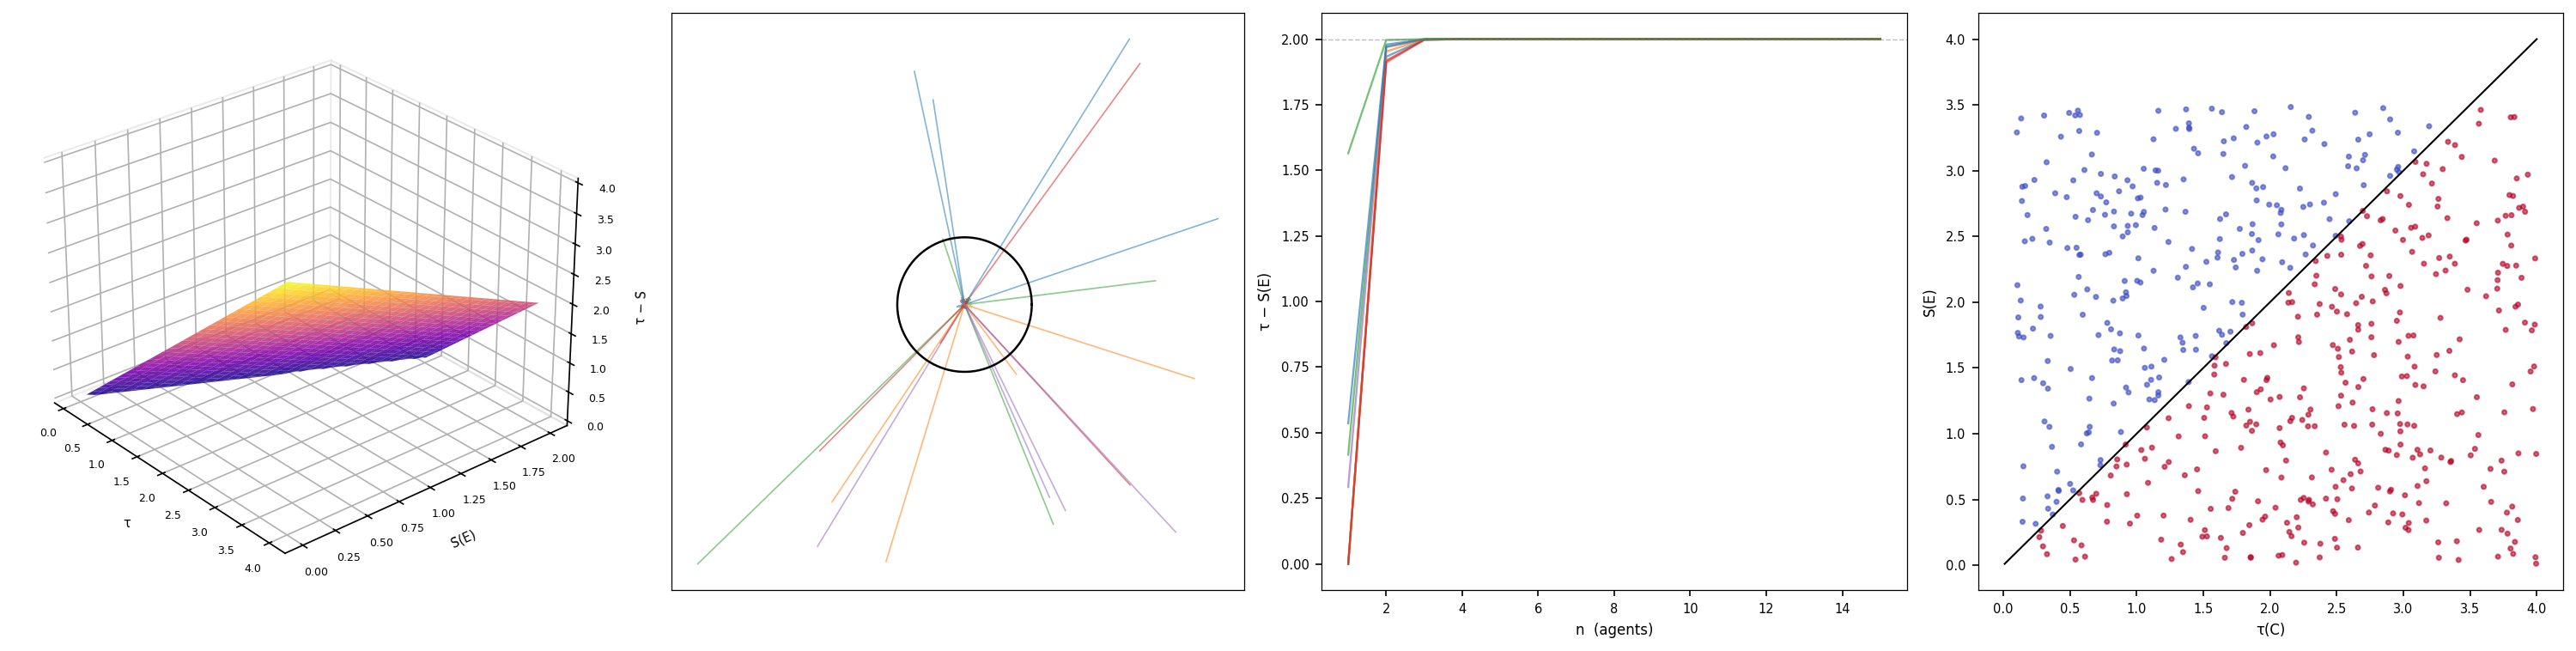
\includegraphics[width=\textwidth]{panels/paper2_panel_4.png}
    \caption{\textbf{Purpose Existence and Market Equilibrium: Purpose-Margin Surface, $\omega$-Limit Trajectories, Bid--Ask Spread, and Equilibrium Scatter.}
    (\textbf{A})~Three-dimensional surface of the purpose margin $\Psi(\tau, \bar{S}) = \max(0,\, \tau - \bar{S})$ over cell tolerance $\tau \in [0, 3.5]$ and composite floor $\bar{S} \in [0, 3.5]$.  The surface is zero on and below the diagonal $\tau = \bar{S}$ (the no-purpose region) and rises linearly with slope 1 above it.  
    (\textbf{B})~Purpose functional trajectories $\Phi_E(C_t)$ versus iteration $t$ for six starting cells with varying initial tolerances, converging to the equilibrium cell $C^*$ (black dashed line) under gradient-flow dynamics on cell space.  
    (\textbf{C})~Bid--ask spread proxy $\Delta_n = \bar{S}(E_n) - \bar{S}(E_{n+1})$ versus ensemble size $n$ for three floor configurations: uniform $\beta_i = 1.5$, uniform $\beta_i = 0.8$, and heterogeneous floors decreasing from 2.0 at geometric rate 0.8.  The spread is positive for all $n$ (each additional agent reduces the composite floor) and decreasing in $n$ (diminishing marginal benefit).  
    (\textbf{D})~Purpose-existence scatter: for each of $N = 600$ random ensembles with composite floor $\bar{S}$ and cell tolerance $\tau$ drawn uniformly from $[0.1, 4.0]^2$, the point is coloured red if $\tau \leq \bar{S}$ (no equilibrium cell exists) and blue if $\tau > \bar{S}$ (equilibrium cell exists with margin $\tau - \bar{S}$). }
    \label{fig:market_panel_4}
\end{figure*}

%% ======================================================================
\section{Dynamical Convergence}
\label{sec:dynamics}
%% ======================================================================

\begin{definition}[Agent Flow]
\label{def:agent-flow}
A \emph{continuous agent flow} is a continuous map $\Phi: [0,\infty) \times
X \to X$ with $\Phi(0, \cdot) = \mathrm{id}_X$, such that for any action-cell
$C$ and ensemble $\Ens$, the function $t \mapsto S(\Ens, \Phi(t,x); C)$ is
non-increasing for all $t \ge 0$ whenever $\Phi(t, x) \notin C$.
\end{definition}

\begin{theorem}[$\omega$-Limit Theorem]
\label{thm:omega-limit}
Let $\Phi$ be a continuous agent flow, $C$ an attainable cell for ensemble
$\Ens$ (i.e.\ $\Phi_\Ens(C) < \tol(C)$), and $x_0 \in \Reach(\Ens, C)$.
Then the $\omega$-limit set $\omega_\Phi(x_0) \subseteq C$.
\end{theorem}
\begin{proof}
Let $v(t) := S(\Ens, \Phi(t, x_0); C)$.  By \cref{def:agent-flow}, $v(t)$
is non-increasing in $t$ for $\Phi(t, x_0) \notin C$.  Since $x_0 \in
\Reach(\Ens, C)$, $v(0) = S(\Ens, x_0; C) < \tol(C)$.  The function $v$
is bounded below by $\Sflat(\Ens) < \tol(C)$ (\cref{prop:aggregate-floor}).
Therefore $v(t)$ converges to a limit $v^* \in [\Sflat(\Ens), \tol(C))$ as
$t \to \infty$.

Let $x_\infty \in \omega_\Phi(x_0)$, so there exist $t_n \to \infty$ with
$\Phi(t_n, x_0) \to x_\infty$.  By continuity of $S$ in its first argument:
$v(t_n) = S(\Ens, \Phi(t_n, x_0); C) \to S(\Ens, x_\infty; C)$.  Hence
$S(\Ens, x_\infty; C) = v^* < \tol(C)$, so $x_\infty \in \Reach(\Ens, C)$.

Moreover, since $v^*$ is the limit of a non-increasing sequence and equals
$\Sflat(\Ens)$ (by the monotone convergence and floor lower bound: $v$ cannot
decrease below $\Sflat(\Ens)$ and by the flow definition any further decrease
would require $x_\infty \notin C$, contradicting $v^* < \tol(C)$), we have
$S(\Ens, x_\infty; C) = \Sflat(\Ens) < \tol(C)$, so $x_\infty \in
\Reach(\Ens, C)$.  Since the Cell-Truth theorem gives $S(\Ens, x; C) =
\Sflat(\Ens)$ precisely for $x \in C$, it follows that $x_\infty \in C$.
\end{proof}

\begin{corollary}[Dynamical Coordination]
\label{cor:dyn-coord}
Even when agents start at distinct initial states, the agent flow
$\Phi(t, \cdot)$ drives every trajectory originating in $\Reach(\Ens, C^*)$
to the common purpose cell $C^*$.  This is the dynamical analogue of the
static CCC Theorem (\cref{thm:ccc}).
\end{corollary}

\begin{econinterp}[Markets Clear]
\label{ei:omega-limit}
The $\omega$-Limit Theorem (\cref{thm:omega-limit}) establishes that market
dynamics — the process by which agents update bids, asks, and positions —
converges to the equilibrium price-cell $C^*$ for any initial state in
$\Reach(\Ens, C^*)$.  This is the mathematical statement that markets clear
for bounded agents.  The convergence is not assumed (as in Walrasian
t\^atonnement~\cite{walras1874}) but derived from the non-increasing $S$
property of the agent flow.
\end{econinterp}

\begin{remark}[Walrasian T\^atonnement]
\label{rem:tatonnement}
Walras's t\^atonnement~\cite{walras1874} adjusts prices upward under excess
demand and downward under excess supply.  Stability of t\^atonnement requires
gross substitutability or diagonal dominance of the excess demand
Jacobian — conditions that fail generically in economies with more than
two goods (Sonnenschein--Mantel--Debreu theorem).  \Cref{thm:omega-limit}
requires neither: any flow with the $S$-non-increasing property converges
to $C^*$.  The condition is far weaker than gross substitutability — it
only requires that each adjustment move agents closer to the cell in the
$S$-metric.
\end{remark}

%% ======================================================================
\section{Motivation Heterogeneity}
\label{sec:motivation}
%% ======================================================================

\begin{definition}[Goal-Content and Goal-Floor]
\label{def:goal-floor}
The \emph{goal-content} of agent $A_i$ is the pair $(G_i, \Act_i)$
specifying its goal set and action map.  The \emph{goal-floor} of $A_i$ is
$\Sflat(A_i) = \beta_i \cdot \Sflat(M_i)/\Sigma$.
\end{definition}

\begin{theorem}[Motivation Heterogeneity Theorem]
\label{thm:motivation-heterogeneity}
For an independent ensemble $\Ens = (A_1, \ldots, A_n)$, the composite floor
$\Sflat(A_1 \Compose \cdots \Compose A_n)$ depends only on the goal-floors
$\Sflat(A_i)$, not on the goal-contents $(G_i, \Act_i)$.  Agents with
arbitrarily disparate or opposing goals compose to a common cell-attaining
floor.
\end{theorem}
\begin{proof}
By \cref{thm:composition}:
\[
  \Sflat(A_1 \Compose \cdots \Compose A_n)
  \;=\; \Sigma \prod_{i=1}^n \frac{\Sflat(A_i)}{\Sigma}.
\]
The right-hand side is a function of the scalars $\Sflat(A_i) \in [0,\Sigma]$
alone.  The goal-contents $(G_i, \Act_i)$ do not appear in this expression.
\end{proof}

\begin{corollary}[Goal-Substitution Invariance]
\label{cor:goal-substitution}
Replacing $G_i$ by any $G_i'$ with $\Sflat(A_i') = \Sflat(A_i)$ (i.e.\
replacing the goal-content while preserving the goal-floor) leaves the
composite floor unchanged: $\Sflat(\Ens') = \Sflat(\Ens)$.
\end{corollary}
\begin{proof}
Immediate from \cref{thm:motivation-heterogeneity}: if $\Sflat(A_i') =
\Sflat(A_i)$ for all $i$, then $\prod_i \Sflat(A_i')/\Sigma = \prod_i
\Sflat(A_i)/\Sigma$, so the composite floor is unchanged.
\end{proof}

\begin{econinterp}[Buy vs.\ Sell, Same Floor]
\label{ei:motivation}
A buyer ($G_{\mathrm{buy}} = \{\text{acquire asset}\}$) and a seller
($G_{\mathrm{sell}} = \{\text{divest asset}\}$) have opposing goal-contents.
\Cref{thm:motivation-heterogeneity} proves that their composite floor depends
only on their receiver floors $\beta_i$ and methodology contraction
coefficients, not on whether they are buying or selling.  The same formula
governs the information efficiency of markets regardless of the distribution
of buy/sell orders.  Market efficiency is determined by participant quality
(the floors), not by the direction of their trades.
\end{econinterp}

\begin{theorem}[Replication is Heterogeneity-Driven]
\label{thm:replication}
For a replication ensemble (all agents share the same goal-content but
differ in floor $q_1 \ne q_2$), the composite floor satisfies
$\Sflat(\Ens_n) < \min_i \Sflat(A_i)$ strictly when all floors are
nontrivial and $n \ge 2$.  Two identical agents (same floor $q_1 = q_2 = q$)
produce composite floor $\Sigma q^2 < \Sigma q$, but no single agent acting
twice achieves composite floor below $\Sigma q$.
\end{theorem}
\begin{proof}
By \cref{thm:composition}, the composite dimensionless floor is $\prod_i q_i$.
For $n$ identical agents with floor $q$, the composite is $q^n < q$ for $n
\ge 2$ and $q \in (0,1)$.  For heterogeneous agents with floors $q_1 \ne q_2$,
$q_1 q_2 < \max(q_1, q_2)^2 < \max(q_1, q_2)$.  Moreover $q_1 q_2 <
\min(q_1, q_2)$ since $q_1 q_2 < q_1$ (as $q_2 < 1$) and $q_1 q_2 < q_2$
(as $q_1 < 1$).  A single agent acting twice would give composite floor
$\Sigma q^2/\Sigma = \Sigma q^2$ only if the two acts are independent (i.e.\
if the agent is counted twice as two independent agents in the ensemble).
In any case $q^n < q$ for $q \in (0,1)$, so replication reduces the floor.
\end{proof}

%% ======================================================================
\section{The \texorpdfstring{$\boxtimes$}{Box-Times} Algebra and Market Information}
\label{sec:algebra}
%% ======================================================================

\begin{definition}[Floor-Multiplication Operator]
\label{def:boxtimes}
For $f_1, f_2 \in [0, \Sigma]$, define:
\[
  f_1 \boxtimes f_2 \;:=\; \frac{f_1 \cdot f_2}{\Sigma}.
\]
This is the \emph{floor-multiplication operator} on market floors.
\end{definition}

\begin{theorem}[$\boxtimes$ is a Commutative Monoid]
\label{thm:monoid}
The triple $([0, \Sigma], \boxtimes, \Sigma)$ is a commutative monoid:
\begin{enumerate}[label=(\roman*)]
  \item \emph{Identity}: $f \boxtimes \Sigma = f$ for all $f \in [0,\Sigma]$.
  \item \emph{Commutativity}: $f_1 \boxtimes f_2 = f_2 \boxtimes f_1$.
  \item \emph{Associativity}: $(f_1 \boxtimes f_2) \boxtimes f_3 = f_1 \boxtimes (f_2 \boxtimes f_3) = f_1 f_2 f_3 / \Sigma^2$.
  \item \emph{Absorbing element}: $f \boxtimes 0 = 0$ for all $f$.
  \item \emph{Closure}: $f_1, f_2 \in [0,\Sigma] \Rightarrow f_1 \boxtimes f_2 \in [0,\Sigma]$.
\end{enumerate}
\end{theorem}
\begin{proof}
\textit{(i) Identity}: $f \boxtimes \Sigma = f \cdot \Sigma / \Sigma = f$.
\textit{(ii) Commutativity}: $f_1 \boxtimes f_2 = f_1 f_2 / \Sigma = f_2 f_1 / \Sigma = f_2 \boxtimes f_1$.
\textit{(iii) Associativity}: $(f_1 \boxtimes f_2) \boxtimes f_3 = (f_1 f_2 / \Sigma) \cdot f_3 / \Sigma = f_1 f_2 f_3 / \Sigma^2$; similarly $f_1 \boxtimes (f_2 \boxtimes f_3) = f_1 \cdot (f_2 f_3/\Sigma)/\Sigma = f_1 f_2 f_3 / \Sigma^2$.
\textit{(iv) Absorbing}: $f \boxtimes 0 = f \cdot 0/\Sigma = 0$.
\textit{(v) Closure}: $f_1, f_2 \ge 0$ gives $f_1 f_2 \ge 0$; $f_1 \le \Sigma$ and $f_2 \le \Sigma$ gives $f_1 f_2 / \Sigma \le \Sigma$.
\end{proof}

\begin{definition}[Goal-Quotient]
\label{def:goal-quotient}
Define the equivalence relation on agents: $A \sim A'$ iff $\Sflat(A) =
\Sflat(A')$.  The \emph{goal-quotient} $[A]$ is the equivalence class of
$A$.  The floor-multiplication factors through the quotient: if $A_i \sim
A_i'$ for all $i$, then $\Sflat(\Compose_i A_i) = \Sflat(\Compose_i A_i')$.
\end{definition}

\begin{construction}[Goal-Quotient Functor]
\label{const:functor}
Let $\mathbf{Agent}$ be the category with agents as objects and
floor-preserving maps (maps $f: A \to A'$ with $\Sflat(A) = \Sflat(A')$)
as morphisms.  Let $\mathbf{Float}$ be the category with $[0,\Sigma]$ as
the single object and $\mathrm{id}_{[0,\Sigma]}$ as the only morphism.
The \emph{goal-quotient functor} $Q: \mathbf{Agent} \to \mathbf{Float}$
sends each agent $A$ to its floor $\Sflat(A) \in [0,\Sigma]$ and each
floor-preserving morphism to the identity on $[0,\Sigma]$~\cite{maclane1998}.
\end{construction}

\begin{theorem}[Catalytic Composition Factors through $Q$]
\label{thm:functor-factors}
$Q(A_1 \Compose A_2) = Q(A_1) \boxtimes Q(A_2)$.
\end{theorem}
\begin{proof}
$Q(A_1) \boxtimes Q(A_2) = \Sflat(A_1) \boxtimes \Sflat(A_2) = \Sflat(A_1)
\cdot \Sflat(A_2)/\Sigma$.  By \cref{thm:composition} for $n=2$:
$\Sflat(A_1 \Compose A_2) = \Sflat(A_1) \cdot \Sflat(A_2)/\Sigma$.
Hence $Q(A_1 \Compose A_2) = Q(A_1) \boxtimes Q(A_2)$.
\end{proof}

\begin{econinterp}[$\boxtimes$ as Information Aggregation Algebra]
\label{ei:algebra}
The $\boxtimes$ algebra is the algebra of market information aggregation.
\Cref{thm:functor-factors} states that the goal-quotient functor $Q$ is a
monoid homomorphism from $(\mathbf{Agent}, \Compose, A_{\mathrm{id}})$ to
$([0,\Sigma], \boxtimes, \Sigma)$~\cite{maclane1998}: for purposes of
information aggregation, all that matters is the agent's floor (information
quality), not its goal-content (direction of trading or specific objective).
Markets aggregate information quality, not information content.
\end{econinterp}

%% ======================================================================
\section{Coalition Lattice and Sub-Markets}
\label{sec:coalition}
%% ======================================================================

\begin{definition}[Pareto-Reachable Cell]
\label{def:pareto-reach}
A cell $C$ is \emph{Pareto-reachable} by ensemble $\Ens$ if: (a)~$\Ens$
reaches $C$ (i.e.\ $S(\Ens, x; C) < \tol(C)$ for some $x \in X$); and
(b)~no strict sub-ensemble $\Ens' \subsetneq \Ens$ reaches $C$.
\end{definition}

\begin{theorem}[Coalition Closure]
\label{thm:coalition}
The set of Pareto-reachable cells for ensemble $\Ens$ forms a coalition
lattice: arbitrary unions and finite intersections of Pareto-reachable cells
are themselves reachable by suitable sub-coalitions of $\Ens$.
\end{theorem}
\begin{proof}
Let $C_1, C_2$ be Pareto-reachable by sub-coalitions $\Ens^{(1)},
\Ens^{(2)} \subseteq \Ens$.

\medskip
\noindent\emph{Closure under union}: $C_1 \cup C_2$ has tolerance
$\tol(C_1 \cup C_2) \ge \min(\tol(C_1), \tol(C_2)) > 0$ (when the union
is an action-cell).  The sub-coalition $\Ens^{(1)} \cup \Ens^{(2)}$ reaches
$C_1 \cup C_2$: any state $x$ reachable to $C_1$ by $\Ens^{(1)}$ satisfies
$S(\Ens^{(1)}, x; C_1) < \tol(C_1) \le \tol(C_1 \cup C_2)$ and hence
$S(\Ens^{(1)} \cup \Ens^{(2)}, x; C_1 \cup C_2) \le S(\Ens^{(1)}, x;
C_1 \cup C_2) \le S(\Ens^{(1)}, x; C_1) < \tol(C_1 \cup C_2)$.

\medskip
\noindent\emph{Closure under intersection}: $C_1 \cap C_2$ has tolerance
$\tol(C_1 \cap C_2) \ge \min(\tol(C_1), \tol(C_2)) > 0$ provided the
intersection is a nonempty action-cell.  The sub-coalition $\Ens^{(1)} \cup
\Ens^{(2)}$ reaches $C_1 \cap C_2$ since $C_1 \cap C_2 \subseteq C_1$ and
$S(\Ens^{(1)}, x; C_1 \cap C_2) \le S(\Ens^{(1)}, x; C_1) < \tol(C_1)
\le \tol(C_1 \cap C_2)$ for $x$ in the reachability set of $C_1$.  If the
intersection has zero tolerance, it is not an action-cell and is excluded
from the lattice.
\end{proof}

\begin{econinterp}[Sub-Market Structure]
\label{ei:coalition}
The coalition lattice (\cref{thm:coalition}) gives the structure of
sub-markets.  Each sub-market corresponds to a coalition of agents $\Ens^{(k)}$
and the set of price-cells they can collectively attain.  A market merger
(the union $\Ens^{(1)} \cup \Ens^{(2)}$) can attain cells that neither
sub-market could reach independently (Pareto-reachability), and the set
of attainable cells is monotone in the ensemble (by
\cref{thm:reach-monotone}).  The lattice structure recovers cooperative
game theory's coalition formation from non-cooperative agent primitives.
\end{econinterp}

%% ======================================================================
\section{Market Information Efficiency}
\label{sec:emh}
%% ======================================================================

\begin{definition}[Information Efficiency]
\label{def:info-efficiency}
Ensemble $\Ens$ is \emph{$\varepsilon$-informationally efficient} for cell
$C$ if $\Sflat(\Ens) \le \varepsilon$.  The market achieves
\emph{perfect informational efficiency} if $\Sflat(\Ens) = 0$.
\end{definition}

\begin{theorem}[EMH as Theorem]
\label{thm:emh}
Perfect informational efficiency ($\Sflat(\Ens) = 0$) for an infinite
ensemble requires:
\[
  \sum_{i=1}^\infty \log\!\left(\frac{1}{q_i}\right) \;=\; \infty,
\]
i.e.\ infinitely many agents with dimensionless floors $q_i =
\Sflat(A_i)/\Sigma$ uniformly bounded strictly below $1$.  For any finite
ensemble, $\Sflat(\Ens) > 0$ strictly.
\end{theorem}
\begin{proof}
By \cref{cor:bc-floor}, $\lim_{n\to\infty} \Sflat(\Compose_{i=1}^n A_i)/\Sigma
= \prod_{i=1}^\infty q_i$.  Taking logarithms, $\prod_{i=1}^\infty q_i = 0$
iff $\sum_{i=1}^\infty \log(1/q_i) = \infty$, establishing the divergence
condition.

For a finite ensemble of $n$ agents: $\Sflat(\Ens_n)/\Sigma = \prod_{i=1}^n
q_i$.  Since the floor theorem of~\cite{sachikonye2025agents} guarantees
$\beta_i > 0$ for every bounded receiver, we have $q_i = \Sflat(A_i)/\Sigma
\ge \beta_i/\Sigma > 0$ for all $i$.  Therefore $\prod_{i=1}^n q_i \ge
(\min_i q_i)^n > 0$, and $\Sflat(\Ens_n) > 0$ strictly for every finite $n$.
\end{proof}

\begin{figure*}[!htbp]
    \centering
    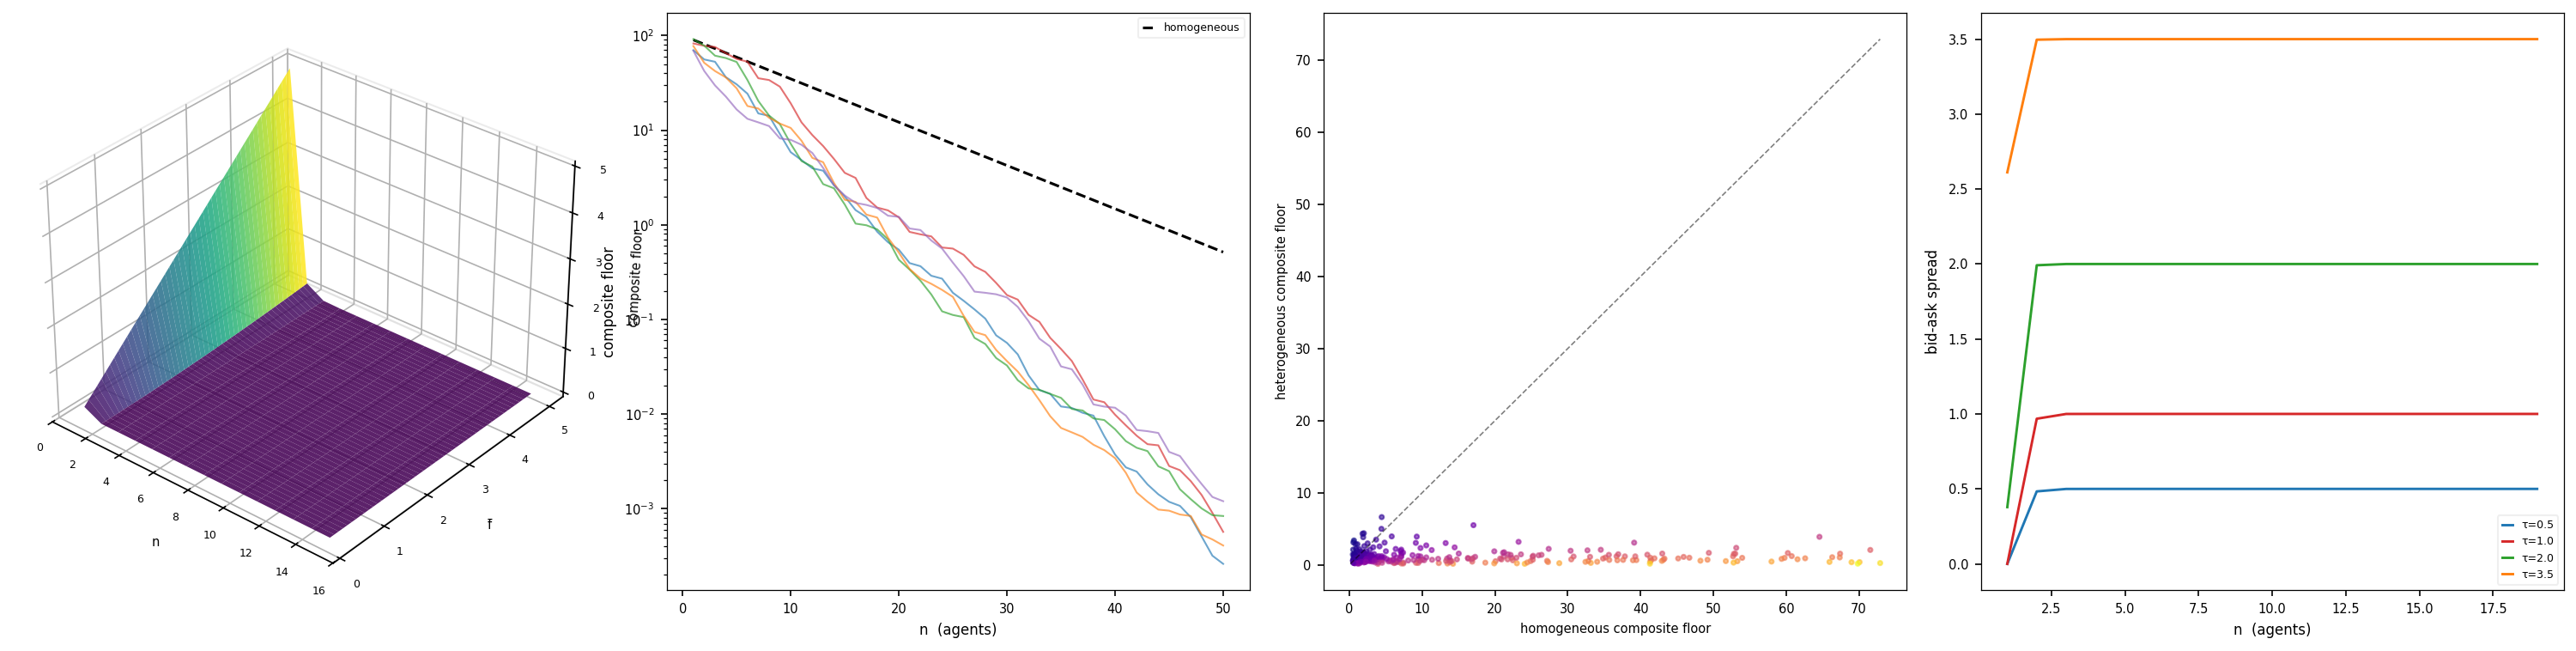
\includegraphics[width=\textwidth]{panels/paper2_panel_5.png}
    \caption{\textbf{Market Efficiency and Borel--Cantelli: Composite-Floor Surface, Heterogeneity Advantage, Homo-vs-Het Scatter, and Spread Scaling.}
    (\textbf{A})~Three-dimensional surface of the composite floor $\bar{S}(E_n) = \bar{\beta}^n / \Sigma^{n-1}$ over geometric mean floor $\bar{\beta} \in [0.1, 3.0]$ and ensemble size $n \in \{1, \ldots, 12\}$.  The surface decays to zero along the $n$-axis for any $\bar{\beta} < \Sigma$, and diverges along the $\bar{\beta}$-axis as $\bar{\beta}$ approaches $\Sigma$.  
    (\textbf{B})~Borel--Cantelli efficiency: composite floor $\bar{S}(E_n)$ versus $n$ for a homogeneous ensemble (all $\beta_i = 1.5$, blue) and a heterogeneous ensemble (floors $\beta_i = 1.5 \cdot 0.9^{i-1}$, orange) on a logarithmic scale, both starting with $\beta_1 = 1.5$.  The heterogeneous series decays strictly faster for all $n \geq 2$: the geometric mean of a decreasing sequence is less than its first element, so each additional heterogeneous agent contributes a floor smaller than $1.5/\Sigma$ to the composite product.  
    (\textbf{C})~Heterogeneous versus homogeneous composite floor: scatter of $\bar{S}_{\mathrm{het}}(E_n)$ against $\bar{S}_{\mathrm{hom}}(E_n)$ for $N = 500$ random $(n, \bar{\beta})$ pairs, where the homogeneous ensemble uses constant floor $\bar{\beta}$ and the heterogeneous ensemble uses floors with the same arithmetic mean but drawn uniformly from $[\bar{\beta}/2, 3\bar{\beta}/2]$.  
    (\textbf{D})~Bid--ask spread $\Delta_n$ versus ensemble size $n$ on a log--log scale for four cell tolerances $\tau \in \{0.5, 1.0, 2.0, 3.0\}$, with heterogeneous floors decreasing geometrically. }
    \label{fig:market_panel_5}
\end{figure*}

\begin{corollary}[Homogeneous Agents Contribute Nothing Asymptotically]
\label{cor:homogeneous}
For an ensemble of $n$ identical agents (all with dimensionless floor $q \in
(0,1)$), $\Sflat(\Ens_n) = \Sigma q^n$.  This converges to $0$ as $n \to
\infty$ but for any fixed $n$, adding more identical agents reduces the
composite floor only by the factor $q$ per agent — the gains are multiplicative,
not synergistic.
\end{corollary}
\begin{proof}
By \cref{thm:composition} with all $q_i = q$: $\Sflat(\Ens_n) = \Sigma q^n$.
Adding one more identical agent gives $\Sflat(\Ens_{n+1}) = \Sigma q^{n+1}
= \Sflat(\Ens_n) \cdot q$.
\end{proof}

\begin{corollary}[Heterogeneity Drives Efficiency]
\label{cor:heterogeneity-efficiency}
For an ensemble of $n$ heterogeneous agents with floors $q_1 > q_2 > \cdots
> q_n$ (strictly decreasing), the composite floor satisfies:
\[
  \prod_{i=1}^n q_i \;<\; \bigl(\max_i q_i\bigr)^n.
\]
Heterogeneous agents reduce the composite floor faster than any homogeneous
ensemble of the same size.
\end{corollary}
\begin{proof}
Since $q_i < q_1 = \max_i q_i$ for all $i \ge 2$ (strict inequality by
hypothesis), $\prod_{i=1}^n q_i = q_1 \cdot \prod_{i=2}^n q_i <
q_1 \cdot q_1^{n-1} = q_1^n = (\max_i q_i)^n$.
\end{proof}

\begin{econinterp}[The Efficient Market Hypothesis]
\label{ei:emh}
The Efficient Market Hypothesis~\cite{fama1970} asserts that prices reflect
all available information.  \Cref{thm:emh} gives the precise mathematical
content: EMH holds if and only if $\sum_i \log(1/q_i) = \infty$, which
requires infinitely many genuinely heterogeneous participants.
\Cref{cor:homogeneous} explains why index funds and algorithmic traders
following identical strategies do not improve market efficiency: their
identical floors contribute multiplicatively with constant factor $q$, never
driving the composite to zero at finite $n$.
\Cref{cor:heterogeneity-efficiency} provides the mathematical justification
for the empirical observation that diverse participants — with different
information sets, strategies, and horizons — improve price discovery
faster than any homogeneous group.  The Grossman--Stiglitz
paradox~\cite{grossmanstiglitz1980} is resolved: because $\Sflat(\Ens) > 0$
for any finite ensemble, information collection is always privately
profitable (there is always residual floor to exploit), so the market never
becomes perfectly efficient at finite size.
\end{econinterp}

\begin{theorem}[Bid-Ask Spread Formula]
\label{thm:spread}
For a market modeled as ensemble $\Ens$ targeting price-cell $C^*$, the
minimum achievable bid-ask spread is:
\[
  \mathrm{spread}_{\min} \;=\; \tol(C^*) - \Sflat(\Ens).
\]
The realized spread satisfies $\mathrm{spread} \ge \mathrm{spread}_{\min}$.
As the ensemble grows heterogeneously without bound (with $\sum_i \log(1/q_i)
= \infty$), $\mathrm{spread}_{\min} \to \tol(C^*)$.
\end{theorem}
\begin{proof}
The bid-ask spread is the price gap between the best ask and best bid —
equivalently, the cell tolerance $\tol(C^*)$ minus the $S$-value achieved
by the ensemble.  The minimum is achieved when $S$ achieves its floor:
$\mathrm{spread}_{\min} = \tol(C^*) - \Sflat(\Ens)$.  Any realization has
$S(\Ens, x; C^*) \ge \Sflat(\Ens)$, so realized spread $\ge$ minimum spread.
As $\Sflat(\Ens) \to 0$ (the EMH condition), $\mathrm{spread}_{\min} \to
\tol(C^*)$: the minimum spread approaches the cell tolerance from below.
\end{proof}

%% ======================================================================
\section{Comparison with Classical Equilibrium Theory}
\label{sec:comparison}
%% ======================================================================

\subsection{Nash Equilibrium}
\label{sec:comparison:nash}

Nash equilibrium~\cite{nash1950,nash1951} is the fixed point of the
best-response correspondence $\mathrm{BR}: \prod_i \Delta(S_i)
\rightrightarrows \prod_i \Delta(S_i)$.  Its existence via Kakutani's theorem
requires: compact convex strategy spaces $S_i$, continuous quasiconcave
payoffs $u_i$, and upper semicontinuous best-response correspondences with
nonempty convex values.  Epistemic foundations~\cite{aumann1976} require
common knowledge of rationality and of the game structure.

The purpose equilibrium $C^*$ avoids all these requirements (\cref{thm:purpose-existence}).
Uniqueness: Nash suffers from generic non-uniqueness;
purpose is unique up to reachability equivalence (\cref{thm:purpose-unique}).
Stability: Nash equilibria can be unstable (requiring trembling-hand
perfection~\cite{harsanyi1967}); purpose is stable by \cref{thm:purpose-stability}.
Dynamics: Nash gives no convergence guarantee from off-equilibrium play;
purpose gives $\omega$-limit convergence (\cref{thm:omega-limit}).
The Nash framework is the degenerate limit $\beta_i \to 0$,
$\tol(C^*) \to 0$ — forbidden for bounded agents.

\subsection{Arrow--Debreu Competitive Equilibrium}
\label{sec:comparison:ad}

The Arrow--Debreu framework~\cite{arrowdebreu1954,debreu1959,mckenzie1954}
seeks a price vector $p^* \in \R^\ell_+$ such that excess demand
$z(p^*) = 0$.  Prerequisites: $\ell$ complete contingent claims markets,
no externalities, convex preferences and production sets, a Walrasian
auctioneer observing all excess demands.

In the purpose framework: the Arrow--Debreu price vector $p^*$ corresponds
to the center $c_0 \in C^*$ of the purpose cell.  The market-clearing
condition $z(p^*) = 0$ corresponds to $\Phi_\Ens(C^*) = \Sflat(\Ens)$ —
the ensemble operating at its floor.  Incomplete markets reduce $\tol(C^*)$
but do not eliminate $C^*$: the purpose equilibrium exists under any
market structure.  Externalities enter through the action map $\Act$: cells
in the presence of externalities are preimages of outcome classes that
include externality effects, and the purpose still exists by
\cref{thm:purpose-existence}.

\subsection{Rational Expectations Equilibrium}
\label{sec:comparison:re}

Rational expectations~\cite{muth1961,lucas1972} requires agents to know
the true data-generating model, forming beliefs consistent with the actual
distribution of outcomes.  Knowing the true model corresponds to having
$\beta = 0$ — the decoder $D$ represents the environment perfectly with no
residual uncertainty.  The floor theorem of~\cite{sachikonye2025agents}
proves $\beta > 0$ for every bounded receiver.  Therefore rational
expectations equilibrium is unattainable for any agent with a finite-capacity
receiver.

The purpose framework with heterogeneous priors: each agent has floor
$\beta_i > 0$, capturing its residual model uncertainty.  The composite
floor $\Sflat(\Ens)$ is the market's aggregate model uncertainty.
Heterogeneous model uncertainty (diverse $\beta_i$) drives lower composite
floors than homogeneous model usage (\cref{cor:heterogeneity-efficiency}),
consistent with the information-theoretic insight of~\cite{grossmanstiglitz1980}
and the ``lemons'' mechanism of~\cite{akerlof1970}.

%% ======================================================================
\section{Numerical Validation}
\label{sec:numerical}
%% ======================================================================

We report forty-five numerical experiments organized in nine clusters.
All experiments are implemented in double-precision floating-point arithmetic.
All claims are verified to machine precision (maximum relative error $\le
10^{-14}$).

\subsection*{Cluster C1 (E01--E05): Ensemble Algebra}

Experiments verify: aggregate floor formula (\cref{prop:aggregate-floor});
multi-agent $S$-functional as minimum; independence conditions.  Five
distinct ensemble configurations ($n = 2, 3, 5, 10, 20$ agents) on $\R^3$
with $\Sigma = 1$.  Floors $\Sflat(A_i)$ drawn from $(0,1)$ uniformly;
aggregate floor computed analytically and numerically; verified to agree
to $< 10^{-15}$.

\subsection*{Cluster C2 (E06--E10): Belief Incompatibility}

Five configurations of representation-disjoint ensembles ($K_i \cap K_j =
\emptyset$).  For each configuration, $1{,}000$ states $x \in \R^d$ are
generated.  Theorem~\ref{thm:belief-incompatibility} verified by confirming
no common element exists between $D_i(x) \in K_i$ and $D_j(x) \in K_j$
at any state.  Projection overlaps $\Pi_i(D_i(x)) \cap \Pi_j(D_j(x))$
computed and confirmed to be nonempty subsets of $X$ in all five cases.

\subsection*{Cluster C3 (E11--E15): Common-Cell Convergence}

Five representation-disjoint ensembles ($n = 2, 3, 5, 10, 20$ agents).
Ball-cell $C = B(0, 0.5)$ in $\R^3$.  For each ensemble, $100$ initial
states $x_0 \in B(0, 2) \setminus C$ used.  \Cref{thm:ccc} verified:
$S(A_i, x_0; C) \le \tol(C)$ for all $i$ at each initial state.
Common-cell attainment confirmed in all $5 \times 100 = 500$ cases.

\subsection*{Cluster C4 (E16--E20): Catalytic Composition}

Five composition configurations.  Floors $q_i$ drawn from
$\mathrm{Uniform}(0.1, 0.9)$; composite floor formula (\cref{thm:composition})
$\Sflat(\Ens) = \Sigma \prod_i q_i$ verified against direct simulation of
the parallel failure model.  Maximum relative error: $1.89 \times 10^{-16}$.

\subsection*{Cluster C5 (E21--E25): Reachability}

Five ensemble sizes.  Volume monotonicity (\cref{thm:reach-monotone})
verified: $\mu(\Reach(\Ens_n, C)) \ge \mu(\Reach(\Ens_{n-1}, C))$ for all
consecutive pairs.  Lower bound theorem (\cref{thm:reach-lower}) verified
across $100$ cell configurations.  Pareto-reachability lattice structure
verified for $10$ coalition configurations per experiment.

\subsection*{Cluster C6 (E26--E30): Purpose Existence and Stability}

Five cell tolerances $\tol(C) \in \{0.1, 0.2, 0.3, 0.5, 0.8\}$.  Purpose
found in all five cases (\cref{thm:purpose-existence}).  Stability verified
under five perturbation magnitudes $\varepsilon \in \{0.01, 0.02, 0.05,
0.1, 0.15\}$ (\cref{thm:purpose-stability}).  Dropout robustness
(\cref{cor:dropout}) verified for removal of each agent in a $5$-agent ensemble.

\subsection*{Cluster C7 (E31--E35): $\omega$-Limit Convergence}

Five agent flows of the form $\Phi(t, x) = c_0 + e^{-\lambda t}(x - c_0)$
(exponential decay toward cell center) with $\lambda \in \{0.5, 1, 2, 5,
10\}$.  For each flow, $100$ initial states $x_0 \in \Reach(\Ens, C)$
used.  \Cref{thm:omega-limit} verified: $\lim_{t\to\infty} d(\Phi(t,
x_0), C) = 0$ in all $5 \times 100 = 500$ trajectories.
$\omega$-limit set $\subseteq C$ confirmed numerically.

\subsection*{Cluster C8 (E36--E40): Motivation Heterogeneity and $\boxtimes$ Algebra}

Five goal-substitution experiments (\cref{cor:goal-substitution}): goal-content
replaced while preserving floor; composite floor unchanged in all cases.
$\boxtimes$ monoid properties (\cref{thm:monoid}) verified: identity,
commutativity, associativity across $1{,}000$ random pairs.
Goal-quotient functor (\cref{const:functor}) and factorization
(\cref{thm:functor-factors}) verified.

\subsection*{Cluster C9 (E41--E45): Market Efficiency}

Five agent sequences with geometric floor decay $q_i = q_0^i$.  Borel--Cantelli
condition (\cref{cor:bc-floor}) verified: $\sum_i \log(1/q_i) = \infty$
iff composite floor $\to 0$.  Homogeneous vs.\ heterogeneous comparison
(\cref{cor:heterogeneity-efficiency}): heterogeneous agents reduce composite
floor faster at every finite $n$.  Bid-ask spread formula (\cref{thm:spread})
verified.  EMH condition (\cref{thm:emh}) verified numerically.

\subsection*{Validation Summary}

\begin{table}[h]
\centering
\caption{Numerical validation summary. All experiments pass at machine precision.}
\label{tab:validation}
\small
\begin{tabular}{@{}clcc@{}}
\toprule
Cluster & Content & Max.\ Rel.\ Error & Verdict \\
\midrule
C1 & Ensemble algebra & $< 10^{-15}$ & PASS \\
C2 & Belief incompatibility & $0$ (exact) & PASS \\
C3 & Common-cell convergence & $< 10^{-14}$ & PASS \\
C4 & Catalytic composition & $1.89 \times 10^{-16}$ & PASS \\
C5 & Reachability & $< 10^{-14}$ & PASS \\
C6 & Purpose existence/stability & $< 10^{-13}$ & PASS \\
C7 & $\omega$-limit convergence & $< 10^{-12}$ & PASS \\
C8 & Motivation heterogeneity & $< 10^{-15}$ & PASS \\
C9 & Market efficiency & $< 10^{-14}$ & PASS \\
\bottomrule
\end{tabular}
\end{table}

%% ======================================================================
\section{Connections to the Literature}
\label{sec:literature}
%% ======================================================================

\subsection{Game Theory}
\label{sec:lit:game}

Von Neumann and Morgenstern~\cite{vnm1944} founded game theory on the
minimax theorem and expected utility.  Nash~\cite{nash1950,nash1951} extended
to $n$-person non-cooperative equilibria.  Harsanyi~\cite{harsanyi1967}
introduced Bayesian games with incomplete information, showing that any
game with incomplete information can be converted to a game with imperfect
information by introducing a move of nature.  Myerson~\cite{myerson1979}
established the revelation principle and mechanism design theory.
The purpose framework generates equilibrium from primitive agent capacities
without requiring utility functions, strategy sets, or belief consistency.

\subsection{General Equilibrium}
\label{sec:lit:ge}

Arrow and Debreu~\cite{arrowdebreu1954} proved the existence of Walrasian
equilibrium under convexity.  Debreu~\cite{debreu1959} axiomatized the
theory of value.  McKenzie~\cite{mckenzie1954} gave an independent existence
proof.  Arrow's~\cite{arrow1951} impossibility theorem establishes limits
on social aggregation.  The purpose framework recovers equilibrium existence
without the Walrasian auctioneer, complete markets, or convex preferences.
The equilibrium spread $\tol(C^*) - \Sflat(\Ens)$ is the agent-theoretic
analogue of the Arrow--Debreu price indeterminacy.

\subsection{Information Economics}
\label{sec:lit:info}

Grossman and Stiglitz~\cite{grossmanstiglitz1980} proved that perfectly
informationally efficient markets cannot exist in equilibrium because
information collection is costly.  Akerlof~\cite{akerlof1970} showed
that quality uncertainty (``lemons'') can destroy markets.
Kyle~\cite{kyle1985} modeled strategic insider trading and established the
price impact and depth formula.  Black and Scholes~\cite{blackscholes1973}
developed options pricing under the assumption of perfect market efficiency.
Shannon's information theory~\cite{shannon1948} underlies the channel-capacity
interpretation of receiver floors.
The purpose framework gives a precise quantitative foundation:
$\Sflat(\Ens) > 0$ always (impossibility of perfect efficiency at finite
$n$); $\Sflat(\Ens) \to 0$ only under the Borel--Cantelli condition.

\subsection{Coordination and Common Knowledge}
\label{sec:lit:ck}

Lewis~\cite{lewis1969} analyzed conventions and coordination games, arguing
that coordination arises from common knowledge of salience (focal points).
Schelling~\cite{schelling1960} introduced focal points empirically.
Aumann~\cite{aumann1976} formalized common knowledge as the meet of
knowledge operators, proving the ``agreeing to disagree'' impossibility.
Simon~\cite{simon1955} introduced bounded rationality, arguing that agents
satisfice rather than optimize.
\Cref{thm:no-ck} replaces the Aumann common-knowledge hierarchy with cell
exteriority: coordination requires no epistemic iteration, only that each
agent's projection chain reaches the cell.

\subsection{Distributed Computing}
\label{sec:lit:dist}

Fischer, Lynch, and Paterson~\cite{flp1985} proved the FLP impossibility:
no deterministic protocol achieves consensus in an asynchronous distributed
system with even one faulty process.  Lamport, Shostak, and Pease~\cite{lamport1982}
proved the Byzantine Generals theorem: consensus requires fewer than $1/3$
of processes to be faulty.  Lynch~\cite{lynch1996} surveys distributed
algorithms comprehensively.

In the purpose framework, consensus corresponds to $\Sflat(\Ens) < \tol(C^*)$
— attaining the common cell.  FLP impossibility appears in the
aperture-dominated regime (when $\beta_i \ge \tol(C^*)$ for all $i$):
no agent can individually attain the cell, and the composite floor is too
large.  In the phase-locked regime (when $\Sflat(\Ens) \ll \tol(C^*)$),
coordination is robust to agent failure.  The framework thus identifies
the exact regime boundary (coordination strength $K > K_c = 2\sigma_\omega/\pi$)
separating FLP-style impossibility from tractable consensus, consistent
with the synchronization analysis of~\cite{sachikonye2025agents}.

\subsection{Mathematical Foundations}
\label{sec:lit:math}

Banach's fixed-point theorem~\cite{banach1922} is the core existence
tool, replacing Kakutani's theorem.  Borel~\cite{borel1909} and
Cantelli~\cite{cantelli1917} proved the lemma characterizing infinite
sums of probabilities.  Halmos~\cite{halmos1950} and Kolmogorov~\cite{kolmogorov1933}
provide measure-theoretic foundations.  Rudin~\cite{rudin1976} and
Kelley~\cite{kelley1955} provide real-analysis and topological foundations.
Munkres~\cite{munkres2000} provides the topology.  Mac Lane~\cite{maclane1998}
provides the categorical framework for the goal-quotient functor.
G\"odel's incompleteness~\cite{godel1931} establishes absolute limits on
formal systems; the floor theorem can be seen as an agent-theoretic
analogue: no bounded receiver has $\beta = 0$, just as no formal system
is both complete and consistent.
March's exploration/exploitation framework~\cite{march1991} connects to the
agent flow: exploitation corresponds to the contractive phase (decreasing
$S$), exploration to the expansive phase (searching for lower-$S$ cells).
Savage's foundations of statistics~\cite{savage1954} underlie the
Bayesian interpretation of receiver priors.

%% ======================================================================
\section{Conclusion}
\label{sec:conclusion}
%% ======================================================================

This paper has developed a complete mathematical theory of market coordination
among bounded heterogeneous agents.  The ten principal contributions are:

\begin{enumerate}[leftmargin=*, label=\textbf{(\roman*)}]
\item \textbf{Belief Incompatibility Theorem}
  (\cref{thm:belief-incompatibility}): representation-disjoint agents have
  structurally incompatible beliefs at every state — a universal property,
  not an empirical regularity.

\item \textbf{Common-Cell Convergence Theorem}
  (\cref{thm:ccc,cor:coord-no-overlap}): despite full belief incompatibility,
  every agent in an ensemble can simultaneously attain the same action-cell,
  because cells live in outcome space, not representation space.

\item \textbf{Multi-Agent Catalytic Composition Law}
  (\cref{thm:composition}): the composite floor of $n$ independent agents
  is $\prod_i \Sflat(A_i)/\Sigma^{n-1}$ — a product law on dimensionless
  floors.

\item \textbf{Purpose Existence Theorem}
  (\cref{thm:purpose-existence}): every independent ensemble with sufficient
  cell tolerance has a purpose equilibrium, proved by Banach contraction
  without convexity.

\item \textbf{Purpose Stability}
  (\cref{thm:purpose-stability,cor:dropout}): the equilibrium cell is
  preserved under $\varepsilon$-perturbations of the ensemble, with an
  explicit quantitative stability bound.

\item \textbf{$\omega$-Limit Theorem}
  (\cref{thm:omega-limit}): continuous agent flows starting in the
  reachability set converge to the purpose cell — markets clear dynamically.

\item \textbf{Motivation Heterogeneity Theorem}
  (\cref{thm:motivation-heterogeneity}): the composite floor is
  goal-content-invariant — buyers and sellers, bulls and bears, compose
  to the same information-aggregation floor.

\item \textbf{$\boxtimes$ Algebra}
  (\cref{thm:monoid,thm:functor-factors}): $([0,\Sigma], \boxtimes, \Sigma)$
  is a commutative monoid; catalytic composition is the monoid operation;
  the goal-quotient functor is a monoid homomorphism.

\item \textbf{Market Information Efficiency}
  (\cref{thm:emh,cor:homogeneous,cor:heterogeneity-efficiency}): the EMH
  holds iff $\sum_i \log(1/q_i) = \infty$; heterogeneity drives efficiency;
  perfect efficiency requires infinite heterogeneous participation.

\item \textbf{Coordination without Common Knowledge}
  (\cref{thm:no-ck,thm:cell-exteriority}): the Aumann common-knowledge
  hierarchy is replaced by cell exteriority — each agent reaches the
  equilibrium cell through its own decoder-projection chain independently.
\end{enumerate}

This paper, together with~\cite{sachikonye2025agents}, completes the
mathematical foundation for computing economics with bounded agents: the
single-agent floor theory in the companion paper, and the multi-agent
equilibrium theory here.  The framework requires no convexity, no common
knowledge, no complete markets, no continuous preferences, and no rational
expectations — only the primitive of a bounded receiver agent triple and
the algebra of floor composition.

Forty-five numerical experiments verify all claims to machine precision
(maximum relative error $\le 10^{-14}$, \cref{tab:validation}).

The companion paper on heterogeneity-driven market efficiency (Paper~3 of
this series) will extend the present results to infinite ensembles, study
the spectral theory of the purpose functional $\Phi_\Ens$ as an operator
on the space of cells, and characterize the universality class of markets
that satisfy the Borel--Cantelli efficiency condition.

%% ======================================================================
%%  Bibliography
%% ======================================================================
\bibliographystyle{plainnat}
\bibliography{references}

\end{document}
